% !Mode:: "TeX:UTF-8"%確保文檔utf-8編碼

\documentclass[11pt,oneside]{book}


\newlength{\textpt}
\setlength{\textpt}{11pt}
    
\newcommand{\flypage}[1]{\begin{titlepage}\begin{center}\vspace*{\stretch{1}}#1\vspace*{\stretch{1}}\end{center}\end{titlepage}}
    
%========基本必备的宏包========%
\RequirePackage{calc,float,multicol,moresize}
%\RequirePackage[onehalfspacing]{setspace}
\linespread{1.5}
%1.3 onehalfspacing
%试卷或需要文字紧凑的
%1.6 doublespacing

%===========加入目录 某章或某节=====%
\makeatletter

\newcommand{\addchtoc}[1]{
        \cleardoublepage
        \phantomsection
        \addcontentsline{toc}{chapter}{#1}}

\newcommand{\addsectoc}[1]{
        \phantomsection
        \addcontentsline{toc}{section}{#1}}

%===========全文基本格式==========%
\setlength{\parskip}{1.6ex plus 0.2ex minus 0.2ex}   %段落間距
\setlength{\parindent}{\textpt * \real{2}}

%=========页面设置=========%
\RequirePackage[a4paper, %a4paper size 297:210 mm
  bindingoffset=10mm,%裝訂線
  top=35mm,  %上邊距 包括頁眉
  bottom=30mm,%下邊距 包括頁腳
  inner=10mm,  %左邊距or inner
  outer=10mm,  %右邊距or  outer
  headheight=10mm,%頁眉
  headsep=15mm,%
  footskip=15mm,%
  marginparsep=10pt, %旁註與正文間距
  marginparwidth=6em,includemp=true% 旁註寬度計入width%旁註寬度
  ]{geometry}

%color
\RequirePackage[table,svgnames]{xcolor}

%================字體================%
%设置数学字体
\RequirePackage{amssymb,amsmath}
\RequirePackage{stmaryrd}
\RequirePackage{fontspec}
%si unit
\RequirePackage{siunitx}
\sisetup{
math-micro = \text{μ},
text-micro = μ
}

\everymath{\displaystyle}

 %設置英文字體
\setmainfont[Mapping=tex-text]{DejaVu Serif}
\setsansfont[Mapping=tex-text]{DejaVu Sans}
\setmonofont[Mapping=tex-text]{DejaVu Sans Mono}

%中文環境
\RequirePackage[]{xeCJK}
\xeCJKsetup{PunctStyle=plain}
\setCJKmainfont[FallBack=DejaVu Serif, ItalicFont=TW-Kai]{Source Han Serif CN}
\setCJKsansfont[FallBack=DejaVu Sans]{Source Han Sans CN}
\setCJKmonofont[FallBack=DejaVu Sans Mono]{TW-Kai}

\RequirePackage{xltxtra} %put here to avoid some package option error. maybe this package is useless ?


%%===============中文化=========%
\renewcommand\contentsname{目~录}
\renewcommand\listfigurename{插图目录}
\renewcommand\listtablename{表格目录}
\renewcommand\bibname{参~考~文~献}
\renewcommand\indexname{索~引}
\renewcommand\figurename{图}
\renewcommand\tablename{表}
\renewcommand\partname{部分}
\renewcommand\appendixname{附录}
\renewcommand{\today}{\number\year{}年\number\month{}月\number\day{}日}


%=======页眉页脚格式=========%
\RequirePackage{fancyhdr}   %頁眉頁腳
\RequirePackage{zhnumber}  %计数器中文化
\pagestyle{fancy}
\renewcommand{\sectionmark}[1]
{\markright{第\zhnumber{\arabic{section}}节~~#1}{}}

\fancypagestyle{plain}{%
    \fancyhf{}
    \renewcommand{\headrulewidth}{0pt}
    \renewcommand{\footrulewidth}{0pt}
    \fancyhf[HR]{\ttfamily \footnotesize \rightmark }
    \fancyhf[FR]{\thepage}}
\pagestyle{plain}


%=========章節標題設計=========%
\RequirePackage{titlesec}
%修改part
\titleformat{\part}{\huge\sffamily}{}{0em}{}
%修改chapter
\titleformat{\chapter}{\LARGE\sffamily}{}{0em}{}
%修改section
\titleformat{\section}{\Large\sffamily}{}{0em}{}
%修改subsection
\titleformat{\subsection}{\large\sffamily}{}{0em}{}
%修改subsubsection
\titleformat{\subsubsection}{\normalsize\sffamily}{}{0em}{}


%================目录===============%
%toc label to contents space   dynamic adjust
\RequirePackage{tocloft}%
\renewcommand{\numberline}[1]{%
  \@cftbsnum #1\@cftasnum~\@cftasnumb%
}

%==============超鏈接===============%
\RequirePackage[colorlinks=true,linkcolor=blue,citecolor=blue]{hyperref} %設置書簽和目錄鏈接等
\newcommand{\hlabel}[1]{\phantomsection \label{#1}}%某一小段的引用


%=================文字強調=========%
\RequirePackage{ulem} %下劃線,加點
\normalem%normal em , not instead of the uline

\DeclareRobustCommand*{\uwave}%波浪线稍微下移点。
{\bgroup \markoverwith{\lower5\p@\hbox{\sixly \char58}}\ULon}

%modified udot command from the dotuline
\def\udot{\bgroup
  \UL@setULdepth
  \markoverwith{\begingroup
     \advance\ULdepth0.1ex
     \lower\ULdepth\hbox{\kern.25em . \kern.045em}%
     \endgroup}%
  \ULon}

\let\oldemph\emph % Save emph in oldemph
\renewcommand{\emph}[1]{\textcolor{red}{#1}}  

%==================插入圖片=======%
\RequirePackage{wrapfig}
\RequirePackage{graphicx}
\graphicspath{{figures/}}
%change the caption style a little like 1-1
\renewcommand{\thefigure}{\arabic{chapter}-\arabic{figure}}


%==============插入表格========%
\RequirePackage{booktabs}
\renewcommand{\thetable}{\arabic{chapter}-\arabic{table}}
\RequirePackage{caption}
%\renewcommand{\arraystretch}{1.3}
%如果用setspace宏包而不是linespread调整行间距,那么才需要额外的表格行距拉大。

%插入代码
\RequirePackage{fancyvrb} 
\fvset{frame=lines,tabsize=4 ,baselinestretch=1.8, fontsize=\footnotesize}


%minted
\RequirePackage{minted}%


%==========其他宏包===========%
\RequirePackage{tikz} 
\usetikzlibrary{calc}

%========脚注=========%
\newcommand*\circled[1]{%
  \tikz[baseline=(char.base)]\node[shape=circle,draw,inner sep=0.4pt,minimum size=4pt] (char) {#1};}
\newcommand*\circledarabic[1]{\circled{\arabic{#1}}}

\RequirePackage{perpage} %the perpage package
\MakePerPage{footnote} %the perpage package command

\renewcommand*{\thefootnote}{\protect\circledarabic{footnote}}


\renewcommand\@makefntext[1]
{\vspace{5pt}
\noindent
\makebox[20pt][c]{\@makefnmark}
\fontsize{10pt}{12pt}\selectfont #1}

\setlength{\skip\footins}{20pt plus 10pt}
%main body 与脚注之间的距离


%framed环境
\RequirePackage{framed}

\newfontfamily{\ubuntu}[Scale=2]{Ubuntu}
\usepackage{newunicodechar}
\newunicodechar{}{{\ubuntu{}}}


\newenvironment{shici}{
\begin{verse}
\centering\large\hspace{12pt}}
{\end{verse}}

\makeatother

\usepackage{indentfirst} 
 

\title{XeLaTeX 指南}
\author{万泽}
\date{第四次修订版}

\newcommand{\bookcover}[1]{\tikz[remember picture,overlay]{\node[inner sep=0] at (current page.center)
{\includegraphics[width=\paperwidth,height=\paperheight]{#1}}}} 
 
\begin{document}
\frontmatter 
\thispagestyle{empty}

\bookcover{book_cover.png}

\cleardoublepage

\flypage{感谢上天}


\addchtoc{第四次修订版前言}
\chapter*{第四次修订版前言}
第四次修订版除了再次全面审视本书籍的内容之外,最重大的一个改动就是将会引入pandoc从tex文件生成epub电子书籍的支持,这就意味着某些LaTex特有的功能将会慢慢抽离出来,这些内容是不可能被epub或者其他标记语言支持的,比如Tikz制图,比如pdf特有的花哨排版需求等。所以本书xelatex基础部分将更加关注于那些latex作为标记语言很容易被其他标记语言转换识别的部分,其他不是那么容易转换甚至不可能转换的部分将会移动到进阶部分而且不会再从tex源码那里进行输出尝试了,只是用文字或者图片进行说明。

一个总的原则就是不要使用latex那些特有的太过于花哨的特性,本书xelatex基础篇部分讨论的内容基本上latex和epub两边都能兼顾得很好,可能epub那边想要显示的样式会没有,比如你定制了一个自己的罗列环境标签,而在epub那边则总是 \verb+1.+ 之类的,因为epub里面的内容实质上是html,所以这可以通过css来进一步调整,问题不是太大。

关于这部分工作的详细内容整理将会在附录中的利用pandoc输出epub一章 \pageref{ch:pandoc_epub} 中有更详细的讨论说明之。

关于本项目epub的css部分,有些是显示需求然后稍作调整,有些是从bootstrap那里或者不知道是那里抄来的,读者权做参考。


\addchtoc{前言}
\chapter*{前言}
我试图收集整理各方面来的xelatex相关的信息,包括自己的实践经验总结,作为后学者的指南手册。

一切在尊重版权的基础上出于爱好兴趣和相信自由分享的价值原则上进行。

第三次修订版删去了一些繁琐晦涩的内容,让文章变得更简洁明了。然后让文章主体部分的编译和生成是平台无关的,主要就是做了一些针对windows平台下的调整工作。这些平台相关的调整知识都加入附录部分了。

\addchtoc{本书基本结构}
\chapter*{本书基本结构}
全书主要分为五大块:
\begin{description}
\item[1. xelatex基础] 这部分内容会就xelatex或者latex的基础知识内容做全面的整理归类排版,争取做到言简意赅并面面俱到和实用性很强的手册性质。

\item[2. xelatex进阶] 更深入地讨论xelatex的特有的排版问题。

\item[3. xelatex高级篇] 这部分讨论了xelatex更底层的一些知识。

\item[4. xelatex应用篇] 这部分讨论了xelatex在不同领域(比如化学,tikz制图,幻灯片,试卷等等)的应用。

\item[5. 附录] 里面有些内容你可能会很感兴趣。
\end{description}


本文的github地址是:\href{https://github.com/a358003542/xelatex-guide-book}{github.com/a358003542/xelatex-guide-book}



\addchtoc{目录}
\setcounter{tocdepth}{2}    
\tableofcontents


\mainmatter 
\part{xelatex基础}

\chapter{背景知识}
\section{TeX}
以下完全按照wikibook中的latex翻译的。\href{http://en.wikibooks.org/wiki/LaTeX/Introduction}{wikibook-latex}

Tex是一个底层的标记式的编程语言,Donald Knuth发明的排版系统,可以用来排版出很漂亮的文章。当初Knuth看到自己的文章和书籍被排版的丑陋不堪,于是在1977年开发了这个排版引擎,这个引擎深深地改变了出版业,大力扩展了数字打印设备的潜能。1989年Tex支持了8位字符,然后Tex的开发就被冻结了,只限bug的修复。Tex作为一种编程语言,是支持if-else结构的:你能够在里面执行数学运算(他们在编译文件的时候被执行),等等。。不过你会发现要做其他的还是很困难的除了排版文字。Tex对于文章的结构和格式提供了良好的解决方案,使得它成为一个强大的神器。Tex是出了名的稳定,可以运行在各种计算机上,几乎没有bug。Tex的版本是按照$\pi$的序列扩展的,目前到了3.1415926。

\section{关于Knuth教授}
Knuth教授是\TeX 排版系统的发明人,出于内容精简的目的,关于Knuth教授的生平信息删去了,有兴趣的请参看\href{http://zh.wikipedia.org/wiki/%E9%AB%98%E5%BE%B7%E7%BA%B3}{wiki-高德纳}。

\section{LaTeX}
LaTeX是一个宏包,其目的是使作者能够利用一个预先定义好的专业页面设置,从而得以高质量地排版和打印他们的作品。LaTeX 最早是由Leslie Lamport编写的,并使用\TeX 作为其排版系统引擎\cite{lshort}。

\section{XeLaTeX}
关于XeLaTeX第一是文档是UTF-8编码的,第二是它对各种字体多语言输出文章的解决方案是最完美的,第三是LaTeX里面能够用的命令它一般都能用,第四是编译生成pdf文件使用的命令是xelatex什么什么tex文件,第五是需要知道它内置引擎现在一般是xdvipdfmx。


\chapter{beginning}
在\LaTeX 的代码中最重要的是理解各种各样的命令的功能,正是这些各种各样的命令让你输入的文字显得与众不同。比如说我现在在打很长的一段文字,\LaTeX 会自动换行的,而我在这里按下Enter键
,实际上并没有换行的效果。理解这一点很重要,\LaTeX 不同于微软的word软件或者其他openoffice之类,不是采用的所见即所得模式,我在这里打的是奇奇怪怪的东西,但是最后显示出来的却可能是很美观的东西。\LaTeX 的一个设计理念就是所想即所得,它甚至有点偏执地要求你组织好你自己的文章的结构,而这正是\LaTeX 的爱好者所推崇的。

同样在代码中你空 一个格或者空      很多个格都是没有区别的,都是一个空格\footnote{现在中文之间的空格不会显示了,不清楚是xelatex还是xecjk宏包处理的,这样挺好的。然后在epub那里还是会保留一个空格。}。



在\LaTeX 中空一行和空很多行的效果是一样的,都是空一行,表示另起一段。

\LaTeX 的命令用到了一些特殊的符号,所以你就不能按照常规用到它们了,这些符号如下:
\begin{Verbatim}
#  $  %  ^  _   &  {  }  ~ \
\end{Verbatim}
%$

更详细的说明请参见后面的特殊符号一章\ref{sec:symbols} 。

\LaTeX 的命令是case~sensitive的。也就是命令是区分大小写的。

现在我把最基本的代码说明一下,\LaTeX 的代码的通用格式是这样的,\textbackslash{}开头,然后跟上命令符号,然后跟上[],方括号中放的是该命令的可选参数,然后跟上\{\},花括号里面跟的是该命令的必填参数。具体如下:
\begin{Verbatim}
\command[optional parameters]{parameters}
\end{Verbatim}


比如说本文档的第一行:\verb+\documentclass[11pt,oneside]{book}+ ,意思是描述文章模板的类型为book,也就是一本书,除此之外还有article,report,slides类型等,更详细的讨论参见documentclass说明一章\ref{sec:documentclass} 。

然后我们看到第二行代码:\verb+\usepackage{什么宏包}+ ,这个usepackage命令后面跟上你想加载的库文件,等你使用\LaTeX 久了,就会接触到更多的宏包的。

然后后面重要的代码有:
\begin{Verbatim}
\begin{document}

文章内容

\end{document}
\end{Verbatim}


其描述了文档的开始和文档的结束。在文档结束命令之后,你写的任何东西都会被\LaTeX 忽略掉。文档环境里面就写着你的文章的内容。

\section{查看宏包帮助文档}
这个我先讲了,实际上沉下心来阅读文档是最好的学习\LaTeX 的方法了。比如我要查看xeCJK文档,就在终端中输入:

\begin{Verbatim}
texdoc xeCJK
\end{Verbatim}


在texmaker的帮助菜单下面有个功能类似的小插件。

\section{从documentclass说起}
\label{sec:documentclass}
文档刚开始是preamble区域,放着文档的一些配置,从begin\{document\}开始进入正文区,出了end\{document\}这句话之后后面写的什么程序都不管了。document是一个环境,后面我们会接触很多的环境的。

documentclass命令的必选参量有article,report,book, slides,beamer等,一般了解这几个就够用了。他们之间有很多细微的差别,这个后面慢慢了解。

tex有以下文档的分节命令:

\begin{Verbatim}
\part{partname}
\chapter{chaptername}
\section{sectionname}
\subsection{subsectionname}
\subsubsection{subsubsectionname}
\paragraph{paragraphname}
\subparagraph{subparagraphname}
\end{Verbatim}

上面的分节命令如果带上星号,如\verb+\section*{}+ 这样的形式则表示该分节不进入目录,也不编号。

一般paragraph和subparagraph分节不怎么使用,就在文档中一行一行空出来即可。还有subsubsection这个分节也不常使用,因为section之下有subsection已经很好地满足了思想的分级结构。paragraph命令可以构建出类似description环境的效果,不同的是后面不缩进,装载内容容量更大。

所以结合前面book,article分类我在这里为了简单起见约定如下:文档中一个小段落就是subparagraph不需要用命令再标识一次,几个段落构成一个paragraph,这从原则上就是某一个问题的阐述,也就是一个section级别,当我们对某一个课题反复思考之后,积累的资料越来越多,然后我们发现某几个section可以合并起来,这样出现了section和subsection两个级别。目录只需要显示section,如果是大型文档有part的时候可以考虑加入少量的subsection,这样目录才不至于过于庞大反而失去了实用性。这所有的section潜在的一个大的分类是chapter,但是这里不需要写出来,因为这个时候整个文档的级别是article。也就是通常所见的小容量的书小册子,某一个专门课题的讨论就按照article来处理。如果上升到某一个学科不同课题的讨论,那么上面article隐藏的chapter写出来,然后将他们合并为book类,这个时候这个book潜藏的最高级别为part。如果是不同学科的合并书籍那么级别就上升到part了。目录在book类的时候有part写上part,然后chapter和section都显示出来,结构也不会太复杂的。

当然以上讨论只是泛泛而论,你需要根据自己的实际情况来,但总的原则是自己心里应该有一个划分标准,毕竟一本书最有价值的部分就是目录了,如果一本书的目录结构是乱七八糟的那么这本书不值一看。

\subsection{一般的可选项}
\begin{itemize}
\item 10pt,11pt,12pt      设置文档所使用字体的大小,默认是10pt\cite{wikibook-latex} 。
\item a4paper ,letterpaper...      定义纸张的大小,此外还有 a5paper,b5paper,executivepaper,legalpaper等。
\item fleqn       设置该选项将使数学公式左对齐,而不是中间对齐。
\item leqno       设置该选项将使数学公式的编号放置于左侧而不是右侧。
\item titlepage, notitlepage       指定是否在文档标题后开始新一页,article文档类不开始新页,report和book开始。
\item onecolumn, twocolumn       指定LaTeX以单栏或双栏方式排版文档。
\item twoside, oneside       指定LaTeX排版文档为双面或单面格式,article和report默认为单面,book默认为双面。
\item openright, openany       定义chapter开始时仅在奇数页或者随意,book类默认openright,report默认openany,article没有chapter。

\end{itemize}



\section{书籍的通用结构}
通常一本书是由好几部份构成的,包括封面、扉页、书名页、目次、序、内文、补充或参考资料、版权页。

出版的书籍的封面和扉页这里我们不考虑。电子书籍就从书名页开始说起。也就是我们的maketitle命令。这个时候也可以认为书名页作为了通常意义上的封面。maketitle可以生成多页,你可以考虑把版权页也算在里面,因为出版的书籍那个版权页刚好在背面,而电子书籍我觉得版权页还是放到最后面合适一些,当然多页封面你还可以自己加点名言警句页,这个看自己喜好了。

然后接下来是序言部分,自序或者他序都可以。自己编的电子书籍就是自序了,自序内容不宜过长,相当于论文的摘要部分,用最简短的话让别人对这本书有一个大概的印象。

接下来如果有listoftables和listoffigures的就放到这里,这个看个人喜好,似乎现在一般都喜欢放在书后面吧。

然后是tableofcontents,目录。

然后是正文部分,包括引言,前言等。

然后是appendix,附录部分是用来提示一些与内容有关而不便载于正文里的资料。

然后是索引:是针对这本书中重要资料如人名、地名、概念等的查检。将本文的重要概念列出,并注明出现在文中的页次。它是依一定的方法排列,通常中文是按字体的笔划多寡决先后顺序,西文则按字母的顺序排列,以便检查。 通常附录是直接资料,索引则是提供查询资料的线索。(索引主要是方便纸质书检索,我觉得如果一本书如果电子化了还是很容易搜索了,可以不加索引了。)


\section{页码控制}
\label{sec:页码}
frontmatter命令跟在begin document后面,接下来页码为罗马数字。

mainmatter命令放在正文开始的前面,表示页码的阿拉伯数字开始计数。

appendix命令表示附录开始,后面各章节改为字母标记。页码没有变化

backmatter命令放在参考文献或者索引的前面。章节编号关掉,页码没有变化。\footnote{backmatter不能在appendix前面,请参考\href{http://tex.stackexchange.com/questions/20538/what-is-the-right-order-when-using-frontmatter-tableofcontents-mainmatter}{这个网站}。}



\chapter{页面布局}
页面布局最好用\emph{geometry}宏包调节。

\section{geometry宏包详细讨论}
页面布局尺寸由geometry宏包指定,页面布局包含很多参量也就是geometry的可选项,请看下图\ref{fig:geometry-option-one}:

\begin{figure}[H]
\centering
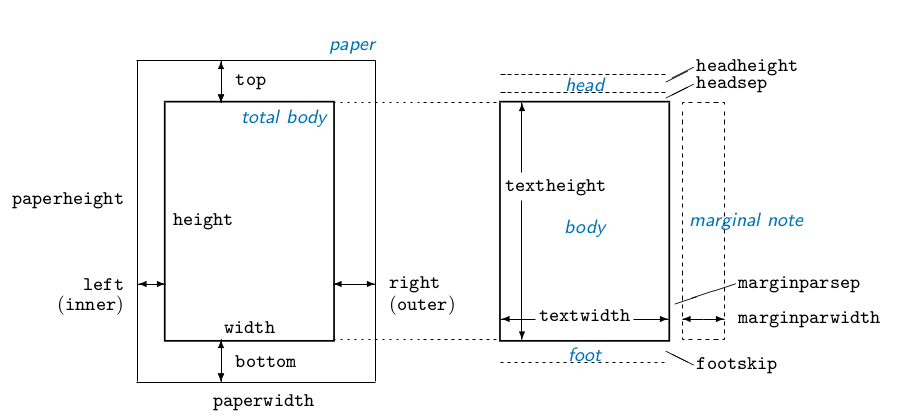
\includegraphics[width=\linewidth ,totalheight=0.95\textheight , keepaspectratio]{geometry-option-one.png}
\caption{geometry选项1}
\label{fig:geometry-option-one}
\end{figure}


geometry提供的纸张类型很多,从a0paper一直到a6paper都有,还有b1paper到b6paper系列等等。纸张类型指定了后面的paperwidth和paperheight就都确定了。

我们先来看横向参量,paperwidth是纸张的宽度,textwidth是正文宽度,marginparsep指旁注和正文之间的间距,marginparwidth指旁注宽度,left指左边空白宽度,right指右边空白宽度。如果book类型是twoside的,那么left最好命名为inner,也就是类似出版书籍靠里面的那段空白宽度,类似的right最好命名为outer,靠外面的那段空白宽度。其中默认情况下width=textwidth,如果加入选项\\includemp=true,那么:\\width=textwidth+marginparsep+marginparwidth。然后还有:\\paperwidth=left+width+right。
\footnote{主要是针对有旁注的情况,在设置为true之后,那么旁注宽度你定义是多少就是多少,左边距右边距是多少就是多少,然后剩下的正文宽度是一个从量(即自动确定的量)了。}

再来看竖向参量,paperheight为纸张高度,textheight是正文高度,top为上面的空白高度,bottom为下面的高度,默认top包含页眉高度headheight和页眉于正文间的一段小空白headsep,bottom包含页脚高度\footnote{这里的概念理清一下,headheight是页眉高度,保证页眉内容能够装的下即可,而headsep是页眉(一般页眉靠下)和正文间的空白距离,也就是你看到的页眉上面的那段空白有top减去headsep再减去headheight剩下的距离,然后这段空白从视觉上来说还有你的页眉文本上面没有填充的部分。而footnote命令插入的文本和页码之间的空白间距是由footskip控制的,然后bottom减去footskip还会得到一个值,这个值是页码下面的空白距离。}footskip和下面的一段空白。所以你的top至少要大于headheight高度。然后中间的区域高度为height。默认情况下height=textheight,请看下图\ref{fig:geometry-option-two}

\begin{figure}[H]
\centering
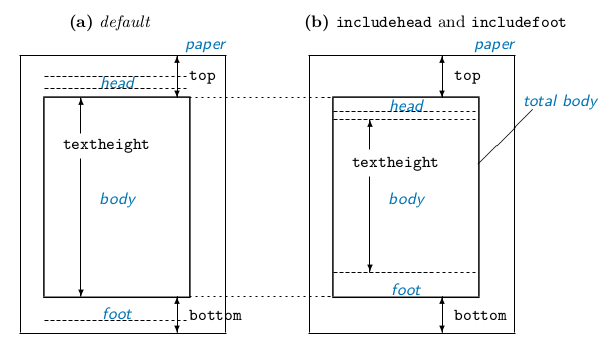
\includegraphics[width=\linewidth ,totalheight=0.95\textheight , keepaspectratio]{geometry-option-two.png}
\caption{geometry选项2}
\label{fig:geometry-option-two}
\end{figure}

如果加上includehead=true选项,那么就和上图右边描述的类似,页眉部分计入height,类似的有includefoot=true,那么页脚部分也计入height。

geometry的机制是以上讨论的横向或者竖向参量指定足够的数量之后,剩下的可以自动计算得到。没有明确指定的参量虽然可以通过计算得到,但是在后面似乎是不能够作为变量使用的?




\chapter{字体}
我们知道xelatex的机制可以调用系统内的任意字体,当然系统没有的字体就要自己安装了(请参看附录ubuntu入门的安装系统字体部分)。

\section{字体的五种属性}
\LaTeX 的字体有五种属性,这五种属性是:字型编码,字族,字型系列,字形,字号,即:encoding,family,series,shape and size。

\subsection{字型编码}
字型编码即各个个别的字在一个字型里头的排列顺序以及安排方式。原始的\TeX 字型编码我们就称为OT1(Old TEX text encoding),这是预设的,如果都不指定字型编码,那所使用的就是OT1编码。在目前新一代的字型编码里头,字的安排方式及内容和OT1不一样,例如T1等。


\subsection{字族}
字族分为三大类,roman or serif(rm),sans serif(sf)和 monospace(tt)。\footnote{下面参考了\href{http://wiki.ubuntu-tw.org/index.php?title=HowtoCustomFontswithFontconfig}{这个网站}}


\begin{description}
\item[serif] Serif中文译为「有衬线字体」,衬线即是印刷字体在每个笔划起始与终止处,加上短线或三角突起等,以便于快速辨认字符,利于阅读,为印刷专用字体。旧版Windows与较旧的Linux发行版以此为预设显示字体,而英文新版则改为Sans-Serif,中文新版则是:当字体大于某一程度时,则将 Serif的明体或宋体,以Sans的黑体取代。

Serif字体著名的有:Times New Roman、DejaVu Serif、宋体、明体等。

\item[sans-serif] Sans-Serif中文译为「无衬线字体」,专用于荧幕、简报、艺术字体、展示等,较美观,但不适于长时间阅读。多数英文语系的作业系统多以此为预设字体,而采用此种字体为预设的中文作业系统,以Mac系统最为著名。

Sans-Serif 字体著名的有:DejaVu Sans、Helvetica、Verdana、圆体、黑体等。

\item[monospace] Mono意思是「单一的」,space 意思是「空间」,中文翻为「等宽字体」。等宽字是打字机时代下的遗产,每个英文字母皆设计为同一宽度,以便于排版;现代为节省不必要空间的浪费,依字母形状分配其宽度,如m与i其宽度便不相同,不相信可以拿尺来量看看。Monospace 现多用于终端机显示、程序码表示等。

Monospace字体著名的有:Andale Mono、DejaVu Sans Mono 、 Courier、AR PL New Sung Mono。
\end{description}


\subsection{字型系列}
正常用的是medium,\textbf{m}。粗体是bold,\textbf{b}。然后还有Bold extended,\textbf{bx}。还有Semi-bold,\textbf{sb}。。和Condensed,\textbf{c}


\subsection{字形}
字形有正常的normal,\textbf{n}。还有意大利斜体Italic,\textbf{it}。斜体Slanted,\textbf{sl}。和Small Caps,\textbf{sc}。


\subsection{字号}
比如说本文设置的就是11pt。



\section{调整五种属性}
\subsection{调整字型编码}
XeLaTeX 只处理UTF-8编码,那个调整字体编码的inputenc和fontenc宏包都不要用了。


\subsection{调整字族}
有两种方法设置,一种是命令式的,一种是环境式的。roman font family是默认的字族,一般不需要明确设置。

\begin{table}[H]
\centering
\begin{tabular}{|c|c|c|}
\hline
命令式 & 环境式 & 描述 \\
\hline
\verb+ \textrm{text}+ & \verb+ {\rmfamily  text}+  & roman字族 \\
\verb+ \textsf{text}+ & \verb+ {\sffamily  text}+  & sans-serif字族 \\
\verb+ \texttt{text}+ & \verb+ {\ttfamily  text}+  & monospace字族 \\
\hline
\end{tabular}
\caption{调整字族}
\label{tab:调整字族}
\end{table}

\subsection{调整字型系列}
默认的medium,一般不需要设置,然后还有一个bold,即字体加粗。

\begin{table}[H]
\centering
\begin{tabular}{|c|c|c|}
\hline
命令式 & 环境式 & 描述 \\
\hline
\verb+ \textmd{text...}+ & \verb+ {\mdseries  text...}+  & 正常字体粗细 \\  
\verb+ \textbf{text...}+ & \verb+ {\bfseries  text...}+  & bold 粗体 \\
\hline
\end{tabular}
\caption{调整字型系列}
\label{tab:调整字型系列}
\end{table}


\subsection{调整字形}
默认是upright shape,常用的字形如下:

\begin{table}[H]
\centering
\begin{tabular}{|c|c|c|}
\hline
命令式 & 环境式 & 描述 \\
\hline
\verb+ \textup{text...}+ & \verb+ {\upshape  text...}+  & 正常字形 \\  
\verb+ \textit{text...}+ & \verb+ {\itshape  text...}+  & 意大利斜体 \\
\verb+ \textsl{text...}+ & \verb+ {\slshape  text...}+  & 斜体 \\
\verb+ \textsc{text...}+ & \verb+ {\scshape  text...}+  & small caps \\
\hline
\end{tabular}
\caption{调整字形}
\label{tab:调整字形}
\end{table}


\subsection{调整字号}
\subsubsection{相对字号调整}
\LaTeX 里面自带的调整相对字号命令如下:
\begin{table}[H]
\centering
\begin{tabular}{|l|l|}
\hline
命令 & 输出\\
\hline
\verb+{\tiny  test line}+ & {\tiny  test line}\\
\verb+{\scriptsize  test line}+ & {\scriptsize  test line}\\
\verb+{\footnotesize  test line}+ & {\footnotesize  test line}\\
\verb+{\small  test line}+ & {\small test line}\\
\verb+{\normalsize  test line}+ & {\normalsize  test line}\\
\verb+{\large  test line}+ & {\large  test line}\\
\verb+{\Large  test line}+ & {\Large  test line}\\
\verb+{\LARGE  test line}+ & {\LARGE  test line}\\
\verb+{\huge  test line}+ & {\huge  test line}\\
\verb+{\Huge  test line}+ & {\Huge  test line}\\
\hline
\end{tabular}
\caption{调整字体大小命令}
\label{tab:调整字体大小命令}
\end{table}

然后我们看下图,不同字号下这些命令确切的大小\footnote{不知道你注意到没有,本文用的是12pt,上面表格上的huge和Huge字号还是有差异,这里因为我加载了moresize宏包的缘故。}:

\begin{table}[H]
\centering
\begin{tabular}{@{}llll@{}}
\toprule 
size          & 10pt (default) & 11pt option & 12pt option \\ \midrule
\textbackslash tiny         & 5pt            & 6pt         & 6pt         \\
\textbackslash scriptsize   & 7pt            & 8pt         & 8pt         \\
\textbackslash footnotesize & 8pt            & 9pt         & 10pt        \\
\textbackslash small        & 9pt            & 10pt        & 11pt        \\
\textbackslash normalsize   & 10pt           & 11pt        & 12pt        \\
\textbackslash large        & 12pt           & 12pt        & 14pt        \\
\textbackslash Large        & 14pt           & 14pt        & 17pt        \\
\textbackslash LARGE        & 17pt           & 17pt        & 20pt        \\
\textbackslash huge         & 20pt           & 20pt        & 25pt        \\
\textbackslash Huge         & 25pt           & 25pt        & 25pt        \\ \bottomrule
\end{tabular}
\caption{字体具体大小}
\label{tab:字体具体大小}
\end{table}


\subsubsection{绝对字号调整}
上面的命令基本上够用了,并不鼓励使用绝对字号。不过有的时候还是有用的,比如旁注环境需要同时调整字体大小和行距,使用这个命令注意不要对文本中某一小段文字使用,否则会造成行距的不一致。
比如这个旁注使用的命令是:

\begin{Verbatim}
\newcommand{\sidenote}[1]{\marginpar{  
 	\fontsize{10pt}{20pt}\selectfont #1}}
\end{Verbatim}

其中fontsize就是调整字号的命令,第一个参量是字体的大小,第二个参量是行距。然后后面\textbackslash selectfont 必须写上,就理解为表示对后面的字体进行操作吧。类似的还有fontencoding,fontfamily,fontseries,fontshape命令,这些本文略过。


\chapter{字体配置}
xelatex字体配置有名的三件套就是:xltxtra,fontspec和xunicode这三个宏包。其中xltxtra宏包是专门处理XeLaTeX 的一些问题的,它会自动加载后面的fontspec和xunicode宏包。xunicode是处理某些特殊字符的。注意xltxtra宏包在加载时我放到所以字体配置宏包的后面,否则会出现错误。下面就字体配置相关宏包详细说明之。


\section{fontspec宏包详解}
当然来自fontspec宏包的帮助文档。后面关于宏包的相关信息来源于自身帮助文档我就不说明了。fontspec宏包主要用于英文字体的设置,中文字体的设置建议用xeCJK宏包来管理。\emph{XeLaTeX 只能使用opentype和truetype字体。}

\subsection{基本的命令}
fontspec宏包最基本的应用就是用setmainfont来设置文档的默认roman字族字体的,setmainfont原来的名字叫setromanfont。\footnote{\href{http://tex.stackexchange.com/questions/70413/problem-with-xetex-latex-and-system-fonts}{参考了这个网站}}setsansfonts是设置文档默认sans-serif字族字体的,setmonofont是设置monospace字族字体的。然后我们看到前面都有一个可选项Mapping=tex-text,这个说是什么让XeTeX 文字分布更好的,可能和正确断行有关系,不大确切。

fontspec宏包有一个和这个宏包名字一样的命令,这个命令非常的基本,大约相当于引擎的入门口,我估计前面三个命令实际上是建构在fontspec命令之上的。fontspec命令的作用不光临时改变字体。还可以加上很多可选项,比如字体尺寸,颜色等等。总之fontspec命令的优先级要高于前面的三大默认字体设置命令。请看下面的例子:

\begin{Verbatim}
{\fontspec[Scale=4,Color=magenta]{Ubuntu} this is a test.} 
\end{Verbatim}

下面显示的是图片,你需要系统安装了ubuntu字体才能运行上面的代码\footnote{ubuntu字体可以在\href{https://design.ubuntu.com/font/}{这里}下载。}。

\begin{figure}[H]
\centering

\includegraphics[width=0.8\linewidth ,totalheight=0.95\textheight , keepaspectratio]{ubuntu_font_show.png}
\end{figure}


另外还有一个有用的命令就是newfontfamily,这个命令相当于把fontspec命令包起来再新建一个命令。新建的那些字体命令就像\verb+\sffamily+之类的命令一样使用。比如加上这一行命令之后:

\begin{Verbatim}
\newfontfamily{\ubuntu}[Scale=3]{Ubuntu}
\end{Verbatim}

后面就可以使用 \verb+\ubuntu{这个命令了}+ 。

以上基本命令总结如下:
\begin{Verbatim}
\fontspec [ font features ] { font name }
\setmainfont [ font features ] { font name }
\setsansfont [ font features ] { font name }
\setmonofont [ font features ] { font name }
\newfontfamily{ cmd }[ font features ] { font name }
\end{Verbatim}

上面的font name在安装字体的时候说明清楚了,比如说用fc-list命令调出来的\textit{宋体,SimSun:style=Regular}中字体名字就是宋体或者SimSun。而在font-manager里面比如第一行显示\textit{Comic Sans MS Regular},字体名就是Comic Sans Ms。接下来主要讨论font features的内容,所讨论的内容以上几个基本命令都适用。由于xeCJK的fontfeatures可选项是继承自fontspec,所以下面的讨论也适用于xeCJK宏包。

\subsection{font features的讨论}
一个字体的字族之下还分为不同的字形,默认的字形设置可能并不能满足你的要求。有一些字体甚至没有粗体或者意大利体这样的字形。一般的玩家就选用默认字形设置足有了,最多在mainfont哪里设置下boldfont和italicfont。比如类似下面这样配置:

\begin{Verbatim}
\setCJKmainfont[BoldFont=Adobe 黑体 Std, ItalicFont=Adobe 楷体 Std]{Adobe 宋体 Std}
\end{Verbatim}

具体字形有:

\begin{Verbatim}
BoldFont = font name
ItalicFont = font name
BoldItalicFont = font name
SlantedFont = font name
BoldSlantedFont = font name
SmallCapsFont = font name
\end{Verbatim}


\subsection{Color}
前面的例子我们看到了Color属性的定制,在这里推荐适用xcolor宏包。XeLaTeX 默认使用的是xdvipdfm,不支持透明颜色。然后xcolor宏包对于颜色的讨论请参看颜色一节\ref{sec:颜色}

\subsection{字体大小}
在前面的那个例子也用到了Scale选项,选个数字来整体调整这个字体的尺寸大小。还有两个常量值,一个是MatchLowercase,一个是MatchUppercase。就是变成小写字母一样的或者大写字母一样的大小。

\subsection{词间距——WordSpace}
觉得默认的设置更有弹性吧,一般的玩家没必要动它。

\subsection{标点后间距——PunctuationSpace}
从零开始可以加点距离。

\subsection{断字符号——HyphenChar}
就是要换行了选择从哪里断字的符号,比如设置HyphenChar={+},那么标明+,就从哪里断字。默认的是\textbackslash{}- 。

\subsection{字母之间的距离——LetterSpace}
从零开始加点距离,而且只适用于小写字母,感觉很累赘。而且这个feature\emph{只适用于XeTeX} 。


\subsection{最后两个命令}
最后还有两个命令defaultfontfeatures和addfontfeatures。有什么优先级:\\ addfontfeatures>fontspec>defaultfontfeatures。觉得太花哨了暂时应该用不到。




\section{设置数学字体}
觉得默认的数学字体也很好看的,就不折腾了。

这里简单提一下,数学没有太多额外需要加载的宏包,其中amssymb和amsmath这两个宏包必备,基本上大家都加载了的。然后数学上或者物理上等对于国际单位和文本中小的数字(但是需要输入上标下标等的)推荐用siuintx宏包处理。

然后通过\verb+\everymath{\displaystyle}+这个语句可以让文本内的数学形式,比如分数显得更大更好看一点。其他问题这里都略过了。

\begin{Verbatim}
\RequirePackage{amssymb,amsmath}
\RequirePackage{fontspec}
%si unit
\RequirePackage{siunitx}
\sisetup{
math-micro = \text{μ},
text-micro = μ
}
\everymath{\displaystyle}
\end{Verbatim}



\section{xeCJK宏包详解}
xeCJK宏包只处理CJK字符在这里指中文字,也就是英文字还是用前面的fontspec宏包来处理。

\subsection{xeCJK宏包的一些命令}
现在对照fontspec宏包对xeCJK新建的只针对CJK字符处理的命令说明如下,其中各个命令的用法和fontfeatures都是类似的。
\begin{description}
\item[setCJKmainfont] 类似于setmainfont。
\item[setCJKsansfont] 类似于setsansfont。
\item[setCJKmonofont] 类似于setmonofont。
\item[CJKfontspec] 类似于fontspec。
\item[newCJKfontfamily] 类似于newfontfamily。
\item[defaultCJKfontfeatures] 类似于defaultfontfeatures。
\item[addCJKfontfeatures] 类似于addfontfeatures。
\item[setCJKmathfont] 估计应该类似于setmathrm。
\end{description}

\subsection{设置CJK字符大小}
可以通过如下命令:
\begin{Verbatim}
\defaultCJKfontfeatures{Scale=1.2}   
\end{Verbatim}
来调整所有CJK字体的属性,比如上面代码的意思就是所有CJK字体都放大1.2倍。比如你在documentclass里面设置10pt,那么实际CJK字符是12pt。\footnote{以前我喜欢放大CJK字体,但是后来发现这样放大之后让数学环境下的字体显得太小很不好看,而且这样整了之后似乎数学环境下的字体也不能通过DeclareMathSizes命令调节了。}


\section{UTF-8编码}
texmaker软件并没有这个问题,不管怎么样,加上这样一行代码没什么害处喽。确保文档以utf-8编码打开和保存。具体就是在文档开头加上如下代码:

\begin{Verbatim}
% !Mode:: "TeX:UTF-8" 
\end{Verbatim}

本文只关注于UTF-8编码。


\chapter{特殊的符号}
\label{sec:symbols}
\section{去掉符号命令后面的空格}
值得一提的是命令如果后面跟上一个花括号,后面的字符紧跟花括号,那么命令显示的符号和后面的字符就没有空格了。比如这里\& a之间就有一个空格,加上花括号\verb+\&{}a+,\&{}a就没有了。

\section{基本的特殊符号}
\subsection{\textbackslash}
\textbackslash ,我们知道命令的开头表示就用它,所以在文档中是不能直接使用的,如果需要显示\textbackslash ,需要输入\textbackslash textbackslash来显示。

\subsection{\{和\}}
\{和\},同上,作为命令的格式。如要显示前面加上\textbackslash 符号。

\subsection{\%}
\% ,我们知道这个符号在文档是用来标记注释信息的开始的,所以在文档也不能直接使用。在前面加个\textbackslash 即可。

\subsection{\~{}}
\~ ,这个符号在文档中产生一格空白,如要显示在前面加上\textbackslash 符号。这样显示的波浪号有点小。还可以进入数学模式下输入\textbackslash sim,在texmaker左边的关系符号一栏中也可以找到。所以为了美观的话就用数学模式吧。然后在Rime输入法里面我们看到还有一种符号是全角下的波浪号~。我比较了下这个和前面两个都不相同,简单起见用这个全角的波浪号也是可以的。——这里所谓的Rime输入法意思就是中文输入法下的全角输入。

\subsection{\$}
\$ ,美元符号之所以不可以用是因为它标记了数学模式的开始和结束。比如说我要输入字母$\pi$,就是在两个美元符号中间输入\textbackslash pi即可。如果直接从输入法输入希腊字母的符号π,这个也是可以正常显示的,只是没有前面数学模式下的美观。我查了一下,数学模式下的那个$\pi$也是unicode区域里面的那个希腊字母,我想只是字体问题了。\footnote{\href{http://www.johndcook.com/unicode_latex.html}{这个网站}用来查找unicode和\LaTeX 命令的对应关系}

\subsection{\#}
\# ,这个符号没怎么接触,latex123说是定义巨集的,前面加上\textbackslash 即可。

\subsection{\^{}和\_{}}
\^{}和\_{},这两个符号表示进入数学模式之后进入上标和进入下标。这两个符号在文本中后面还要跟一对花括号,否则显示会出问题。

\subsection{\&}
\& ,这个符号表示表格中的分隔符。要显示前面加上\textbackslash 即可。

\subsection{单引号和双引号}
你可以用\textbackslash textquotedblleft来表示左双引号,用:\textbackslash textquotedblright 来表示右双引号。用\textbackslash textquoteleft来表示左单引号,用\textbackslash textquoteright来表示右单引号。

然后还有敲键盘的方法,要左边和右边区别对待,比如说左单引号就是点击ESC下面那个键,右单引号是点击分号右边那个键;而左双引号是点两次ESC下面那个键,右双引号是按住shift,然后点击分号右边那个键。

一边单引号和双引号都用全角模式,中文的输入法调试好会很方便输入的,这不存在什么问题。至于英文左单引号和右单引号好像一般不怎么区分。

\subsection{破折号和连字号}
连字号就是一个这个[-] ,可以直接在键盘上输入。\\
短破折号就是两个-连续输入成为→  [--]\\
长破折号就是三个-连续输入成为→  [---]\\
负号如果在数学模式下是→  $ -1 $  如果有时嫌麻烦就直接-1应该可以接受把。

此外中文全角短的连字号有[-],unicode码是U+FF0D;长破折号是[——],有两个unicode码U+2014的符号组成。值得注意的是长破折号的一个,[—],和前面的全角短连字号也是有所不同的,似乎稍微长一点,一般不怎么用吧,但我发现有些书排版有时用到这个符号。

\subsubsection{两个连字号的显示}
比如要显示终端选项的时候有两个短连字号,如果你直接输入两个--就变成短破折号了。如果你要有这样的显示效果,-{}-,那么你需要中间加一个花括号\footnote{\href{http://tex.stackexchange.com/questions/9813/how-can-i-stop-latex-from-converting-two-hyphens-to-a-single-hyphen-when-loading}{参考网站}}。下面是三个连字号的例子:\\
\verb+-{}-{}-+\\
-{}-{}-


\subsection{温度的度}
在texmaker左边的关系负号哪里我们可以看到一个小圆圈,输入命令是\textbackslash circ,当然需要在数学模式下。现在就需要让这个小圆圈位于上标即可。前面的符号介绍我们提及\^{},就是进入上标显示,上标的内容在\^{}后面的那个花括号内,于是我们就知道三十度怎么画了。$ 30^{\circ} $ ,注意texmaker左边有快捷键。点起来很方便的。具体代码是:\$ 30\^{}\{\textbackslash circ\} \$。当然你可以直接用rime输入法打出这个温度的度:°,℃。在输出\%候选项哪里。

\subsubsection{更加专业的做法:}
输入温度的度的更加专业的做法利用siunitx宏包的degreeCelsius命令输出:\verb+30\si{\degreeCelsius} and 45\si{\degree}+

\begin{figure}[H]
\centering
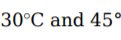
\includegraphics[scale=1 , keepaspectratio]{wendu.png}
\end{figure}

\subsection{省略号}
英文输入法下直接输入三个小数点和使用 \verb+\ldots+ 命令区别不大,中文省略号请使用中文输入法下的全角模式下的省略号。



\chapter{初步中文化}
主要是些原\LaTeX 常量是英文单词,然后改成中文字即可。看看代码就清楚了。
\begin{Verbatim}
\renewcommand\contentsname{目~录}
\newcommand\econtentsname{Contents}
\renewcommand\listfigurename{插图目录}
\renewcommand\listtablename{表格目录}
\renewcommand\bibname{参~考~文~献}
\renewcommand\indexname{索~引}
\renewcommand\figurename{图}
\renewcommand\tablename{表}
\renewcommand\partname{部分}
\renewcommand\appendixname{附录}
\renewcommand{\abstractname}{摘~要}
\renewcommand{\today}{\number\year{}年\number\month{}月\number\day{}日}
\end{Verbatim}

值得一提的是不同的文档类包含不同的命令,比如有的文档类可能没有定义today这个命令,比如article类不包含参考文献命令等。



\chapter{段落}
\section{换行和分段}
一个意思写一个段落,意思没说完就不要分段,在文章中一个段落的书写就是直接写就是了,\LaTeX 会自动处理好一切的。简单的分段的做法就是空一行。这样分段首行缩进仍然存在,表示不同的段落。

如果你只是想换行而不分段,那么用命令 \verb+\\+ 可以满足你的要求。

\textbackslash \textbackslash 命令还有一个用法,比如后面跟上[10pt],表示在原有行距的基础上再加上额外的空白距离,参数也可以是负数。

换行不空一行在tex文档中的效果只是加上一个空格,你可以前面那行后面加上\%{}来取消这个空格。


\section{断字}
如果你编译的时候出现了overfull hbox什么的错误,一般是断字出现问题了,有字越过文档边界了。命令\textbackslash \textbackslash 是强制换行。还有一个换行命令\textbackslash linebreak,这个命令后面还可以跟个可选项,但意义我不大明确。一般就是观察生成的文档,然后选择合适的位置插入linebreak命令。这个断行命令断行之后,前面那行的文字将会扩展充满整行,在越界小距离的情况下还是可行的,但是距离大了这一行扩展导致字间距过大也不是十分美观。

一般断字问题主要是英文单词的断字,你可以在你想要断字的位置加上\verb+\- +,这样系统会自动判断,如果这里适合断字它就会在这里断字,这种断字方法不会加上符号\verb+-+。其实还有一种直接的断字方法,那就是在你想要断字的文字加上\verb+-\\+,这样会显示符号\verb+-+。第三种断字方法就是在你觉得可能要断字的地方加上符号\verb+-+,这样系统会自动判断在那里断字,然后也会显示符号\verb+-+。



\section[段落中的行距]{段落中的行距\footnote{参考了\href{http://www.complang.tuwien.ac.at/anton/latex/baselineskip.html}{这个网站}}}
\label{sec:段落中的行距}

\begin{Verbatim}
\setlength{\baselineskip}{22pt}
\end{Verbatim}


上面的代码就是设置行间距的。一行一行之间的间距也是一个glue,我们知道glue有基本的space和伸缩量。行距的基本space由命令baselineskip控制,伸缩量有baselinestretch命令。\footnote{实际上这个多少有点揣测的意思。}

一般行间距的调整用宏包setspace,似乎这个宏包对文档其他内容比如脚注旁注等都有所调整,但是如果你自己定义的脚注格式就不太依赖这个宏包了。不过用法也简单,如下所示:\\
\verb+\RequirePackage[doublespacing]{setspace}+

此外还有选项onehalfspacing,如果你试了onehalfspacing和doublespacing(当然还有默认的不拉伸间距的情况),你都感觉不太满意。这个时候推荐你使用linespread命令,在刚开始的配置内容里写上即可,不需要额外的宏包加载。其中\verb+\linespread{1.3}+的效果相当于前面的onehalfspacing,如果是1.6则相当于doublespacing,然后当然,1.4,1.5等等都随你设置了。


值得注意的是linespread命令还会对表格有拉伸效果,而setspace宏包没有这个效果。所以如果用setspace宏包而不是linespread调整行间距,那么才需要对arraystretch量进行一些修改,提供额外的表格行间距。


\subsection{baselineskip} 
段落中行之间上下间距\footnote{一行一行就是横向的盒子,行间距就是横向的盒子之间的上下间距。}由三个命令控制:baselineskip,lineskip和lineskiplimit。简单的说明就是首先间距是baselineskip,但是如果上面的盒子伸的太下或者下面的盒子伸的太高,那么他们就可能会碰到一起。lineskiplimit控制的就是盒子之间最小间距,比如0pt。当baselineskip减去上面的盒子的深度depth再减去下面盒子的高度height然后得到的值比lineskiplimit小,那么跳转方案就会选择lineskip模式。也就是上面盒子最低的点和下面盒子最高的点之间的距离是lineskip那么多。\footnote{参看了a beginner's book of \TeX 的spacing between boxes一节。在google book哪里可以看到这一段,不过似乎这本书网上并不能自由下载。}

我感觉自己设置一个baselineskip已经很满足要求了,尤其个别字用Huge命令的时候效果也还行。


\subsection{baselinestretch}
baselinestretch量相当于行间距glue的伸缩量,也就是对前面的baselineskip做一定的伸缩\footnote{参看的\href{http://tex.stackexchange.com/questions/49596/no-effect-of-baselinestretch}{这个网站}}。这个命令要使用的话格式如下:\\
\verb+\renewcommand{\baselinestretch}{伸缩量}+\\
这个命令等价于:\\
\verb+\linespread{伸缩量}+\\
不过这不是故事的全部。如果要在文档中改变行间距必须采用如下的形式:\\
\verb+{\linespread{伸缩量}\selectfont  sometext  \par}+

{\linespread{3} \selectfont 其中伸缩量和前面说的一样是:设为1.3就是1.5倍行距,1.6就是双倍行距,其他自由发挥。除了要封闭环境否则对其他文本有影响外,还需要加上selectfont命令,此外最后还必须加上\textbackslash par命令,否则会没有效果。\par}



\section{段落间距}
\verb+\setlength{\parskip}{1.6ex plus 0.2ex minus 0.2ex}+\\
段落间距也就是一段和一段之间的空白距离。上面就是本文段落间距的设置代码。parskip是一个length量。其中距离设置设置一个固定量和一个加量还有一个减量,wikibook中说很有用,不太清楚。


\section{段首缩进}
\subsection{段首缩进量调整}
\begin{Verbatim}
 \setlength{\parindent}{\textpt * \real{2}}
\end{Verbatim}

上面代码就是设置段首缩进量的,其中parindent是一个length量。具体就是两个字符的意思。这里预先需要加载calc宏包\footnote{注意乘法乘以小数的时候需要用real命令处理。},为了让设置的距离更加相对化,我新建的一个长度量textpt:\\
\verb+\newlength{\textpt}+\\
\verb+\setlength{\textpt}{11pt}+\\ 
本文的默认字体大小值是11pt,然后传递到了textpt这里。


\subsection{章节第一段的缩进}
默认章节第一段是不会缩进的,如果你希望每个章节的第一段也缩进那么就需要加载 \textbf{indentfirst} 宏包即可。如果你希望某一段不缩进就用noindent命令吧。



\section{段落对齐}
flushleft环境为左对齐环境,flashright环境为右对齐环境,center为居中环境。类似的命令样式有raggedleft,raggedright和centering。这些命令还可以控制表格图片(也许是一切盒子?)的位置。简单示例如下:

\begin{Verbatim}
\begin{flushright}
右边才是王道。
\end{flushright}
\end{Verbatim}

\begin{flushright}
右边才是王道。
\end{flushright}


\section{flushright环境空白间距问题}
flushright环境有一个大型的空白间距,如果你不喜欢这么大的空白间距正如前面谈及的,可以使用raggedright等命令来调整,不过raggedright等命令似乎更适合对图片表格等盒子调整位置(raggedright命令不太好用,有时不知怎么不起作用,推荐就用hfill命令让其他内容居右,唯一要提醒的是hfill命令是针对当前行把内容往右推。)

那么在段落内如何实现类似word那种一行之类居右对齐?

\begin{Verbatim}
this is a test line

{\vspace{-\parskip}\hfill  some text}
\end{Verbatim}

这里推荐先空一行分段,然后用hfill命令将文本推到右边去,然后用vspace调整下距离。这里选择-\textbackslash parskip这样得到的行距和其他行距是一致的。

{\vspace{-\parskip}\hfill  然后我注意到开辟新的竖向模式}\\,比如换行之后,不空一行用smallskip,medskip等,然后不用vspace命令调整也是可以的。因为smallskip也是一种vspace命令的调整模式,但是行距和其他的不太一致,所以在这里推荐就空一段,然后负的parskip。当然如果可以接受不用vspace调整也是可以的。



\chapter{页眉页脚设计}
页眉页脚设计推荐用\emph{fancyhdr}宏包。
\section{观察}
我什么都没设置,生成的文档有章名的那一页中间有页码,其他页右上角有页码。有章名的那一节可能样式是plain,其他页可能是默认的myheadings样式。

\section{全部信息归零}
\subsection{plain样式重置}
fancyhdr宏包提供了一个命令fancypagestyle来重新或者定义一个新的页眉页脚样式。现在我将plain样式所有信息全部清除,宁愿没有也不愿出现其他别样的信息。
\begin{Verbatim}
\fancypagestyle{plain}{
    \fancyhf{}
    \renewcommand{\headrulewidth}{0pt}
    \renewcommand{\footrulewidth}{0pt}}
\end{Verbatim}
该代码第一行是提出要重新定义plain样式,然后里面包含新的定义。第二行是所有的页眉页脚信息换为空值,第三行是将页眉那条线宽度设为0pt,也就是不显示了,第四行类似是页脚那根线不显示了。

\subsection{选择默认样式为empty}
使用命令:\\
\verb+\pagestyle{empty}+\\
也就是明确指定页眉页脚样式为已经有的样式empty,即什么都没有。现在文章所有的页眉页脚信息都被清除了。现在摆在我们面前有两条路,一条是继续DIY plain样式,然后全部页面设置为plain样式。一条是plain继续归零,然后自己DIY一个新的样式并使用这个样式。我在这里选择第一条道路了。

\section{继续定制plain样式}
我不太喜欢那一条横线,有需要的请自己将前面的什么rulewidht命令横线宽度设为0.4pt左右。

我是一个喜欢简单的人,fancyhdr宏包里面还有很多命令:
\vspace{-20pt}
\begin{Verbatim}
\lhead[<even output>]{<odd output>}
\chead[<even output>]{<odd output>}
\rhead[<even output>]{<odd output>}
\lfoot[<even output>]{<odd output>}
\cfoot[<even output>]{<odd output>}
\rfoot[<even output>]{<odd output>}
\fancyhead[selectors]{output you want}
\fancyfoot[selectors]{output you want}
\end{Verbatim}
这些命令都可以用fancyhf命令来达到,所以我不做介绍了,有需要的请参考fancyhdr宏包文档。

\subsection{fancyhf命令的可选项}
fancyhf命令的一些可选项如下表所示,比如偶数页的页眉左边位置的表示就是EHL,奇数页页脚中间位置就是OFC。本文没有区分偶数页和奇数页,而且也不想有过多的信息,比如就想页眉左边和页脚右边有点内容,那么可选项为HL和FR。
\begin{table}[H]
\centering
\begin{tabular}{@{}ll@{}}
\toprule
字母 & 意义  \\ \midrule
H  & 页眉(head)  \\
F  & 页脚(foot)  \\
L  & 左边(left)  \\
C  & 中间(center)  \\
R  & 右边(right)  \\
E  & 偶数页(even) \\
O  & 奇数页(odd) \\ \bottomrule
\end{tabular}
\caption{fancyhf可选项字母意义}
\label{tab:fancyhf可选项字母意义}
\end{table}


\subsection{本文页眉页脚配置代码}
\begin{Verbatim}
\RequirePackage{fancyhdr}   %頁眉頁腳
\RequirePackage{zhnumber}  %计数器中文化
\pagestyle{fancy}
\renewcommand{\sectionmark}[1]
{\markright{第\zhnumber{\arabic{section}}节~~#1}{}}

\fancypagestyle{plain}{%
    \fancyhf{}
    \renewcommand{\headrulewidth}{0pt}
    \renewcommand{\footrulewidth}{0pt}
    \fancyhf[HR]{\ttfamily \footnotesize \rightmark }
    \fancyhf[FR]{\thepage}}
\pagestyle{plain}
\end{Verbatim}

首先是加载fancyhdr宏包\footnote{exam类有自己的页眉页脚定制方法,和fancyhdr宏包有冲突。}。接下来是页面风格fancy,不先这样做后面的sectionmark的重定义无效,具体原因不明。

然后接下来重定义sectionmark,这个sectionmark我不太明白,十分有意思的它在exam文档类里面照样有效,但是如果不设置\verb+\pagestyle{fancy}+它就无效,然后放在新定义的plain样式里面也会出错。

下面就是重新定制plain样式,首先是:
\begin{Verbatim}
%    \renewcommand{\chaptermark}[1]
%    {\markboth{第\zhnumber{\arabic{chapter}}章~~#1}{}}
%    \fancyhf[HL]{\ttfamily \footnotesize \leftmark }
\end{Verbatim}
为了文档简洁这些代码我都注释掉了,不过你可能用的着。这里leftmark就是目前的章名,fancyhf带上选项HL就是定义文档页眉左边的内容。然后通过修改chaptermark(如果你章节标题不自己DIY的话,这里修改chaptermark你会看到变化的。)会影响leftmark的内容。这里的markboth也是配套的。

\begin{Verbatim}
    \fancyhf[HR]{\ttfamily \footnotesize \rightmark }
    \fancyhf[FR]{\thepage}
\end{Verbatim}
这里的rightmark就是目前的节名,通过修改sectionmark会影响它的内容。sectionmark的重新定义如前所示是和markright命令配套的。


我起初试图如下重新定义chaptername和sectionname,然后重新定义thechapter和thesection也就是当前章节编号。在这里先将编号用arabic命令转化为1,2,3...的形式,然后用zhnumber命令(来自 \verb+zhnumber+ 宏包)转化为一,二,三...的形式。可是目录形式也跟着改变了,还有图片编号。影响范围太大了,所以就直接用上面代码的形式组合了。


FR也就是右边页脚处,哪里简单填上\textbackslash thepage即表示当前页码。具体格式不用设置,请参看页码这一小节\ref{sec:页码}。

\begin{Verbatim}
\fancyhfoffset[R]{\marginparwidth+\marginparsep}
\end{Verbatim}
最后这段代码可要可不要,作用是让页眉页脚扩展到旁注的宽度那里。放在这里,如果设置marginparwidth和marginparsep都是0pt的话,也没有什么影响的。



\chapter{章节标题设计}
推荐使用\emph{titlesec}宏包进行章节标题设计,当然还有其他的宏包可以设计出更加花哨的章节标题这里忽略。

\section{本文章节标题设计}
\begin{Verbatim}
\usepackage{titlesec}
\titleformat{\part}{\huge\sffamily}{}{0em}{} 
\titleformat{\chapter}{\LARGE\sffamily}{}{0em}{} 
\titleformat{\section}{\Large\sffamily}{}{0em}{}
\titleformat{\subsection}{\large\sffamily}{}{0em}{}
\titleformat{\subsubsection}{\normalsize\sffamily}{}{0em}{}
\end{Verbatim}
本文章节标题设计非常简单,几乎就是titleformat命令各个选项的空值。

\section{titleformat命令说明}
titlesec宏包还提供了其他一些命令,不过一切设置都可以通过titleformat命令来获得:
\begin{Verbatim}
\titleformat{\chapter}[shape]{格式}{label}
    {sep}{before-code}[after-code]
\end{Verbatim}
第一个花括号是选择你要修改的目标,也就是是章啊,还是节啊,还是小节。从part到subparagraph都可以的。

后面是shape,一个可选项,没看懂要干嘛的。估计也不太重要吧。

第二个花括号是重点,里面放着格式命令,比如设置字体字族,字体大小,颜色等都可以的。这个格式影响后面要讲的label标签还有标题文本。\footnote{这里对齐命令,vspace命令等都是可以用的?}

第三个花括号是标签,空着就是没有标签。你也可以──比如说对于section的标题──填上\verb+\thesection+表示节的编号。

第四个花括号是标签和后面标题文字之间的空隙,这里因为没有label所以设为0了,如果有label还是加点距离。

第五个花括号和后面的可选项是什么标题盒子之前和之后的代码,这里忽略。有兴趣请参看文档。


\section{章节编号数值修改}
part,chapter,section等这些都是counter量,\\通过setcounter命令直接修改──比如说section──为2,那么接下来counter自动计数是从2开始,下一个section编号是3。

\section{章节编号深度修改}
通过设置secnumdepth这个counter的量可以设置章节编号深度。\\
\verb+\setcounter{secnumdepth}{1} +\\
默认是2,编号到subsection,你可以设置为3,subsubsection都有编号,或者设置为1,section有编号。我想设置为0的话section也没有编号了。

\section{章节编号形式修改}
\label{sec:章节编号形式修改}
thepart,thechapter,thesection,thesubsection等你可以称他们为标签吧,也就是通常我们看到的编号那部分内容。通过对这些命令重定义就可以对他们进行修改了。\\
\verb+\renewcommand{\thesection}{\arabic{section}.}+\\
那么就会有1. 的形式。

\section{章节标题上插入脚注}
一般使用章节标题命令就是\verb+\section{text}+,前面还是可以加个可选项的,这个可选项的文本将作为目录中实际显示的文本,而后面则是实际执行的文本。比如:\\
\verb+\subsection[text]{{\color{red}    text}\footnote{脚注}}+
\subsection[text]{{\color{red}    text}\footnote{脚注}}



\chapter{目录设计}
一般在封面之后插入目录,用tableofcontents命令即可。本文没有对目录做太多的修改,默认的目录格式挺好的。

\section{目录深度控制}
\verb+\setcounter{tocdepth}{1} +\\
tocdepth是一个counter量,默认是2,显示到subsection。这里为了是目录更加简洁,设置为了1即显示到section。0显示到chapter,-1显示part,-2就什么都没有了。

\section{前言加入目录}
\label{sec:前言加入目录}
本文定义了两个命令为了做到这点:
\begin{Verbatim}
\newcommand{\addchtoc}[1]{  %目录中加入新章节
	\cleardoublepage   
	\phantomsection    
	\addcontentsline{toc}{chapter}{#1}}
\newcommand{\addsectoc}[1]{ %目录中加入新的section
	\phantomsection    
	\addcontentsline{toc}{section}{#1}}	
\end{Verbatim}
两个命令大致类似吧,一个是针对chapter的,一个是针对section的。其中chapter的需要加上一个cleardoublepage命令,其具体解释参看\href{http://www.personal.ceu.hu/tex/breaking.htm#clrdblpage}{这个网站}。意思是首先结束本页,然后将所有图片和表格都显示出来。在两面twoside模式里,要确保下一页从奇数页开始,必要时插入空白页。

后面的phantomsection命令\footnote{这个命令名字真不好记。。}是由hyperref宏包提供的,需要加上它使链接有效。     
\footnote{参看了\href{http://www.forkosh.com/latex/ltx-171.html}{这个网页}}

然后addcontentsline命令就是将目前章节加入目录,第一个花括号里面的选项有:toc,lof,lot。也就是目录,图目录和表目录。第二个花括号里面如果是toc的话就是part,chapter之类的,如果是lof,好吧,一般加入label就可以了,还没接触这种情况,说不上什么。最后那个花括号里面放着要在目录上面显示的文字。

本文目录的前面加入如下命令即可:\\
\verb+\addchtoc{目录}+

同理,参考文献处理情况类似。值得提醒的是section的时候注意换命令。然后part,section之类的命令带个星号*表示不编号不进入目录,这个前面说过的。

\section{目录行间距拉大}
我试图建立一个通用的格式环境横跨目录的时候会失效,只好将其分开。不过这样做带来一个好处,那就是你在目录前面设置一些格式只对目录起作用。比如:\\
\verb+\addtolength{\parskip}{8pt}+\\
这里对段落之间的间距增加了一点宽度,这个会影响一条条目录之间的行间距。


\section{目录编号和标题间距调整}
如果你的目录编号,也就是前面的label和标题内容有点重叠,那么可以用tocloft宏包来自动调整目录编号和标题间距。具体代码如下:
\begin{Verbatim}
\RequirePackage{tocloft}%
\renewcommand{\numberline}[1]{%
  \@cftbsnum #1\@cftasnum~\@cftasnumb%
}
\end{Verbatim}

well,具体看不懂,不过把这段代码加上之后效果确实不错,请参考\href{http://tex.stackexchange.com/questions/64115/table-of-contents-chapter-number-width}{这个网站}。




\chapter{封面设计}
基础的封面就是用title输入题目,用author输入作者,用date命令输入日期,默认是输出当时编辑的日期的。author里面可以用and命令连接几个作者或者用\textbackslash \textbackslash 命令换行。然后用maketitle命令插入一个封面即可。


\section{一个简单的封面}
为了说明基本知识我使用本文早期的一个简单的封面作为例子讲解。
\begin{Verbatim}
%===========%封面設計=====%
\makeatletter
\renewcommand\title[1]{\def\@title{#1}}
\renewcommand\author[1]{\def\@author{#1}}
\newcommand\email[1]{\def\@email{#1}}
\newcommand\version[1]{\def\@version{#1}}
\newcommand\editor[1]{\def\@editor{#1}}

\renewcommand{\maketitle}{
	\begin{titlepage}
	\begin{flushleft}
	
	 \vspace*{\stretch{1}}
    {\Huge\sffamily \@title}\\[10pt]
    {\sffamily\large 作者: \@author}\\
    	
	\vspace{\stretch{1}}
	{\sffamily 編者: \@editor}\\[10pt]
	{\sffamily 郵箱: \href{mailto: \@email}{\@email}}\\
	
	\vspace{\stretch{1}}
	{\large\ttfamily 版本號: \@version}\\[10pt]
	{\large\ttfamily  完成日期: \today}\\
	
	\end{flushleft}
	\end{titlepage}
}
\makeatother
\end{Verbatim}
这个代码一些小的细节我就不说明了,现在就主要内容说明一下。这个封面主要是通过重新定义maketitle命令来完成的,然后前面还加上了一些新的输入命令。其中makeatletter和makeatother一前一后表示他们夹著的内容@这个符号就是一个符号,这样‘@abc’和‘abc’是不同的。

def命令是\TeX 的原始定义命令,比如说:\\
\verb+\newcommand\email[1]{\def\@email{#1}}+\\
就是定义@email命令,然后这个命令的输出就是输出\#{}1。\#{}1也就是第一个参数。也就是email命令接受到的参数。

然后封面设计就是进入titlepage环境进行一些排版操作即可。这里涉及到的居左对齐,vspace等命令就不多说了。

我的建议是一般对封面没什么要求的就用默认的样式或者类似前面的稍作DIY,如果要做出出版级的华丽封面,而且要每本书都不同的话,建议还是用tikz绘图或者其他绘图软件来处理,然后把图片导入即可。毕竟\LaTeX 的设计本意只是日常文档排版。



\chapter{引用}
\section{文章内部引用}
某一个特别的章节图片或者表格等需要被引用时,你就在它哪里加上label命令。然后就可以用ref命令在文章内部建立链接引用他们了。值得一提的是texmaker的提示功能非常好。建立label的时候方便你管理,section部分前面就加一个sec:前缀,图片加一个fig:前缀,表格加个tab:前缀等。然后labe中文英文都是可以的,方便自己管理最好写的很明晰。

比如在这里我插入了一个参考文献的引用,是用的是cite命令。\\
\verb+ \cite{lshort}+请参见文献\cite{lshort}

还有一个pageref命令和ref命令差不多,文档上写法都类似,不同的是在文章上显示的是页码。



\section{hyperref宏包简介}
\subsection{如何插入超链接}
比如这里插入一个超链接到google,\href{https://www.google.com/}{google} 。

首先要在前面加载hyperref库文件:
\begin{Verbatim}
\usepackage{hyperref}
\end{Verbatim}


然后在你想要插入超链接的地方使用命令:

\begin{Verbatim}
\href{https://www.google.com/}{google}
\end{Verbatim}



\subsection{链接字体颜色控制}
\begin{Verbatim}
\usepackage[colorlinks=true,linkcolor=blue,
        ulrcolor=red,citecolor=blue]{hyperref} 
\end{Verbatim}

\textbf{colorlinks=ture}是把颜色打开,如果是false那么都是默认的黑色了。后面的选项主要影响文字颜色,还有更多颜色设置。linkcolor影响目录颜色和脚注和内部引用,ulrcolor影响对外链接,citecolor影响对文献的链接。anchorcolor超链接源码。

hyperref宏包目前我的DIY只限于一些颜色设置,有兴趣的请自己研究\href{http://mirrors.ctan.org/macros/latex/contrib/hyperref/doc/manual.pdf}{文档}。



\chapter{脚注}
加入脚注还是很有用的\footnote{这就是一个脚注}。具体方法就是:

\begin{Verbatim}
\footnote{这就是一个脚注} 
\end{Verbatim}


\section{脚注标签修改}
重定义thefootnote命令会影响每一条脚注前面的label样式,比如默认的1.。
\begin{Verbatim}
\renewcommand{\thefootnote}{\arabic{footnote}}
\end{Verbatim}


\section{一页脚注重新编号}
我喜欢每一页脚注都重新编号,觉得那些数字反正也没什么意义。具体实现如下代码所示。
\begin{Verbatim}
\usepackage{perpage} 
\MakePerPage{footnote} 
\end{Verbatim}


\section{脚注中的距离}
\begin{itemize}
\item \verb+\footnotesep+,长度量, 控制脚注与脚注之间的距离。
\item \verb+\skip\footins+,长度量,控制正文和脚注之间的距离。
\end{itemize}


\section{重定义脚注文本格式}
\begin{Verbatim}
\renewcommand\@makefntext[1]
{\vspace{5pt}
\noindent
\makebox[20pt][c]{\@makefnmark}
\fontsize{10pt}{12pt}\selectfont #1}
\end{Verbatim}

这里重新定义了(在sty文件中)\verb+\@makefntext+命令,命令的参数就是每一条脚注的内容的。都是一些格式的调整,主要的改动是加入了一个盒子放着脚注的标签(\verb+\@makefnmark+)。


\section{表格里的脚注}
\href{http://texblog.org/tag/footnote/}{参考了这个网站},具体实现过程很简单,就是表格放入minipage环境下即可直接使用脚注命令了。

\begin{Verbatim}
\begin{minipage}{6cm}
	\begin{tabular}{|l|c|c|}
		\hline
		A & 1 & 2 \footnote{This is a footnote.} \\
		\hline
		B & 2 & 1 \\
		\hline
		C & 3 & 3 \\
		\hline
	\end{tabular}
\end{minipage}
\end{Verbatim}


\begin{minipage}{6cm}
	\begin{tabular}{|l|c|c|}
		\hline
		A & 1 & 2 \footnote{This is a footnote.} \\
		\hline
		B & 2 & 1 \\
		\hline
		C & 3 & 3 \\
		\hline
	\end{tabular}
\end{minipage}





\chapter{文字强调}
\section{emph命令}
emph命令一般是英文换成斜体,中文换成楷体(也就是前面设置的意大利字形的字体)。不过不同字族会有不同的表现。如果在强调环境之内有强调(一般没有这种情况把。)那么文字又会换成常规形态。
emph命令是\LaTeX 自带的最基本的用于文字强调的方法。


\section{重新定义emph}
\label{sec:emph}
本文档中的emph命令被重新定义了:
\begin{Verbatim}
\renewcommand{\emph}[1]{\textcolor{red}{#1}}  
\end{Verbatim}

比如:\emph{我觉得字体设为红色更加起到强调作用} 。

\section{underline命令}
这个也是\LaTeX 自带的命令,就是加上下划线,不过在中文中并不能正确换行。所以往下看。

\section{ulem宏包}
下面的内容来自ulem宏包。\footnote{现在ulem中文可以正确换行了。}

\subsection{ulem宏包源码}
ulem宏包在ubuntu系统中源码的位置是:

\begin{Verbatim}
/usr/share/texlive/texmf-dist/tex/generic/ulem
\end{Verbatim}

ulem宏包提供如下命令:uline,uuline,uwave,sout, xout,dashline,dotuline。主要用于文字的强调,其中uline是下划线,dotuline是加点强调,uwave是波浪线。其他命令请参看ulem宏包文档。

\uline{这是一段很长的测试文字,主要用于说明中文情况下加入下划线并且能够正确的换行。用的是uline命令。}

注意如果单纯加载ulem宏包,原有的emph命令也会成为类似uline命令的效果,也就是加下划线。可以后面跟上命令\textbackslash normalem,也就是emph命令还是原来的处理效果。



\chapter{插入列表}
itemize和enumerate环境其实也支持item后面跟上可选项的形式,只是从格式上他们常常出界,不建议使用。
\section{基本使用}
\subsection{itemize环境}
\begin{Verbatim}
\begin{itemize}
\item 这是一个列表
\item 这又是一个列表
\end{itemize}
\end{Verbatim}


\begin{itemize}
\item 这是一个列表
\item 这又是一个列表
\end{itemize}



\subsection{enumerate环境}
\begin{Verbatim}
\begin{enumerate}
\item 这是一个列表
\item 这又是一个列表
\end{enumerate}
\end{Verbatim}

\begin{enumerate}
\item 这是一个列表
\item 这又是一个列表
\end{enumerate}

\subsection{description环境}
\begin{Verbatim}
\begin{description}
\item[鸭子]是一种动物
\item[苹果]是红色的
\end{description}
\end{Verbatim}
\begin{description}
\item[鸭子]是一种动物
\item[苹果]是红色的
\end{description}

\section{enumerate环境标签的修改}
\label{sec:enumerate环境标签的修改}
\textbf{NOTICE: } 这里的修改都只是在pdf那边的,epub这边都是默认的形式。

enumerate环境中各个item标签自动生成是依赖各个对应的计数器,然后通过labelenumi,labelenumii,labelenumiii和labelenumiv这几个命令控制的,也就是重新定义这些命令,标签样式就被修改了。这几个中最常用的是第一级标签labelenumi,下面就这个命令给出例子。

首先我希望这个enumerater环境的item计数从0开始,然后我希望它的格式是<0>。

\begin{figure}[H]
\centering

\includegraphics[scale=1 , keepaspectratio]{enumerate_1.png}
\end{figure}



上面的实现实际tex代码如下所示:
\begin{Verbatim}
\begin{enumerate}
\setcounter{enumi}{-1}
\renewcommand{\labelenumi}{<\arabic{enumi}>}
\item 这是一个列表
\item 这又是一个列表
\end{enumerate}
\end{Verbatim}

估计计数器使用的时候都会先加一,所以为了初值为0,只好先设置为-1了。


再举个例子,假设你已经加载了 \textbf{zhnumber} 包了,那么我们可以实现中文中常见的那种罗列环境:

\begin{figure}[H]
\centering

\includegraphics[scale=1 , keepaspectratio]{enumerate_2.png}
\end{figure}


上面的实现实际tex代码如下所示:

\begin{Verbatim}
\begin{enumerate}
\renewcommand{\labelenumi}{\zhnumber{\arabic{enumi}}.}
\item 这是一个列表
\item 这又是一个列表
\end{enumerate}
\end{Verbatim}


\section{itemize环境标签的修改}
itemize环境里面当然没有计数器,不过它类似的也有:\\ labelitemi,labelitemii等命令,通过重定义这些命令就可以影响第一级第二级等标签样式。




\chapter{插入图片}
要插入一个图片,\LaTeX 文档开头那里要加载库文件:
\begin{Verbatim}
\usepackage{graphicx}
\end{Verbatim}


然后在你想要插入图片的地方输入如下命令:
\begin{Verbatim}
\includegraphics[scale=1]{图像名字}
\end{Verbatim}


插入图片有很多参数可以设置,这里就最有用的宽度和高度设置说明一下。具体就是height表示高度,width表示宽度。然后等于多少in(英寸)。参数放在可选参数那里。不过我觉得下面这个参数设置挺实用的,如下:

\begin{Verbatim}

\includegraphics[width=\textwidth, keepaspectratio]{test.png}
\end{Verbatim}

其中\textbackslash textwidth 表示让图片和文本内容区块一般宽,后面经过摸索发现使用linewidth可能更好,因为在多栏环境下linewidth就是那栏的宽度,但这具体读者自己决定了。然后keepaspectratio参数意思是缩放的时候保持宽高比不变。

\section{图片标签的修改}
\label{sec:图片标签的修改}
本文的图片环境标题通过输入 \verb+\caption{text}+ 即实现如下形式的图片标题:\verb+图 1-1: text+  。

其中图这个字是通过重定义figurename命令来完成的。

\begin{Verbatim}
\renewcommand\figurename{图}
\end{Verbatim}


而后面本来默认的是1.1这样的形式,但是常见的都是1-1这样的形式,通过重定义thefigure命令即可达到目的。

\begin{Verbatim}
\renewcommand{\thefigure}{\arabic{chapter}-\arabic{figure}}
\end{Verbatim}

\subsection{取消图片标签}
有时候通过caption插入图片标题,前面的标签你不想要。这个时候就算将thefigure命令设置为控制还是会有“图:”这两个文字,如果这两个你都不想要。推荐用caption宏包的caption*命令,那个命令完全没有标签,写成什么样子显示就是什么样子。


\section{设置图片寻找文件夹}
如下的命令设置,这样\TeX 会自动在这些文件夹寻找文件,也就是你在include图片时直接写上图片文件名即可。这个语句是支持多个文件夹设置的。

\begin{Verbatim}
\graphicspath{{figures/}}
\end{Verbatim}



\section{图片格式的讨论}
\subsection{支持的图片文件格式}
使用xelatex和graphicx宏包,目前我测试支持的图片格式有:eps,png,jpg,pdf。

\textbf{NOTICE:} 但是如果你需要在epub那边也能够正常显示图片,则需要将图片格式限定在jpg或者png中。

\subsection{搜索图片后缀名控制}
经测试上面的eps,png,jpg,pdf格式的图片后缀名默认都支持,也就是只要写上前面的文件名即可。

\textbf{NOTICE:} 为了epub那边也能够正常显示图片,图片的后缀名你需要写上,不能省略。




\section{本文常使用的插入图片代码片段}

\begin{Verbatim}
\begin{figure}[H]
\centering
\includegraphics[scale=1 , keepaspectratio]{fig_name.png}
\end{figure}
\end{Verbatim}

\begin{Verbatim}
\begin{figure}[H]
\centering
\includegraphics[width=\linewidth ,totalheight=0.95\textheight , 
    keepaspectratio]{fig_name.png}
\end{figure}
\end{Verbatim}

上面第一个插入图片例子缩放 \verb+scale=1+ ,这对于那些尺寸较小的图片有不错的显示效果。如果图片较大的话,那么就可以考虑使用第二个代码片段,其使用了 \verb+width=\linewidth+ 来让图片自动适应你的文档的linewidth(之所以选择linewidth是因为在多栏环境下也会自动适应到那个栏的宽度。)。





\chapter{插入表格}
\section{基本情况的讨论}
一般情况下一些小的表格就用tabular环境处理即可。
下面看这个例子:
\begin{Verbatim}
\begin{table}[h]
\centering
\begin{tabular}{|c|c|}
\hline
l & l表示该列格子左对齐 \\
\hline
c & c表示该列格子居中 \\
\hline
r & r表示该列格子右对齐 \\
\hline
\end{tabular}
\caption{tabular参数}
\label{tab:tabular参数}
\end{table}
\end{Verbatim}

例子显示如下:
\begin{table}[H]
\centering
\begin{tabular}{|c|c|}
\hline 
l & l表示该列格子内容左对齐 \\
\hline
c & c表示该列格子内容居中 \\  
\hline
r & r表示该列格子内容右对齐 \\ 
\hline
\end{tabular}
\caption{tabular参数}
\label{tab:tabular参数}
\end{table}
在table环境那里我加了一个可选参数h,意思是在这里就在这里。这个表格还有图片环境都是什么浮动体。我们看到他们可以加上caption命令从而有一个标题,然后table和figure后面有个可选参数来控制这个浮动体的位置。默认是tbp。不过我喜欢用h,也就是在这里如果可能。有的时候h的表现效果可能不太让你满意。那么你可以尝试float宏包,它提供了H参数,会更加强制地控制浮动体,H的意思是一定要在这里。

这段代码中centering命令是让表格居中。caption命令是加上标题,label命令是方便引用。

最重要的就是tabular环境,前面|符号表示画一个竖线,也就是每一列刚开始画一条竖线,你也可以不画表示每一列开始不画竖线。然后是字母c,表示每一列第一个格子居中对齐,类似的还有字母l(left)和r(right)。还有一种格式p{width},表示该格子具有width的宽度,然后里面的文字自动断行。

hline命令表示画一条横线。\& 这个特殊符号表示进入下一列。\textbackslash \textbackslash 表示进入下一行,后面跟上可选项距离,那么下一行的高度将拉高。


\section{booktabs宏包}
如果你只是想要一个简洁明了的表格,目前大家公认的好的表格标准就是三线表式,你也可以称之为booktabs风格吧。简单来说有以下规则\footnote{按照Markus Püschel的small guide to making nice tables里面的介绍。}:

\begin{enumerate}
\item 不要垂直线
\item 不要双横线
\item 每一行的各个格子都有足够的空间
\item 一律左对齐
\item 三线,toprule,midrule,bottomrule
\end{enumerate}


在这里我们还有个捷径\footnote{texmaker编辑器的向导菜单那里有个表格向导方便快速生成表格tex代码片段。},不一定要手工将表格代码全部敲出来。首先我们找一个表格软件,libreoffice的或者gnumeric都行。然后将数据输入进去保存好。然后我们将数据选择复制,打开网站:\href{http://www.tablesgenerator.com/}{http://www.tablesgenerator.com/} ,在那个网站的表格的开头哪里按下Ctrl+v。这个网站还有一些设置可以调整,稍微摸索下就知道了。唯一要说的是那个activate/deactivate custom grid edit选项,可以选择绘制某几根线框显示。在这里不做调整,直接选择最右边的booktabs table style。然后把多余的行或者列删除掉,就可以点击下面的generate了。生成的代码如下:
\begin{Verbatim}
\begin{table}[h]
\begin{tabular}{@{}ll@{}}
\toprule
参数       & 描述       \\ \midrule
l        & 左对齐      \\
c        & 居中       \\
r        & 右对齐      \\
p{width} & 一定宽度自动换行 \\ \bottomrule
\end{tabular}
\end{table}
\end{Verbatim}
表格的显示效果初步如下:
\footnote{你注意到这里有@\{\},意思是每一列前面有一段空白,可以被花括号中的字符填充,这里是完全取消掉那点空白。booktabs的风格是开头那点空白和最后一列最后那点空白全部取消掉。}
\begin{table}[H]
\begin{tabular}{@{}ll@{}}
\toprule
参数       & 描述       \\ \midrule
l        & 左对齐      \\
c        & 居中       \\
r        & 右对齐      \\
p{width} & 一定宽度自动换行 \\ \bottomrule
\end{tabular}
\end{table}

接下来就是微调整了,比如说上面的花括号没有正常显示,还有想要居中,开头加上centering命令,还有caption标题命令,还有label。修改之后结果如下:
\begin{table}[H]
\centering
\begin{tabular}{@{}ll@{}}
\toprule[1.2pt]
参数       & 描述       \\ \midrule
l        & 左对齐      \\
c        & 居中       \\
r        & 右对齐      \\
p\{width\} & 一定宽度自动换行 \\ \bottomrule[1.2pt]
\end{tabular}
\caption{tabular参数-2}
\label{tab:tabular参数-2}
\end{table}

\section{一个三线表模板}
这是一个简单的三线表模板,你可以在texmaker或者其他编辑器里面设置好快速插入代码片段的功能。然后快速输入一下代码块,然后填上数据,这样就很快捷了。
\begin{Verbatim}
\begin{table}[H]
\centering
\label{tab:}
\caption{}
\medskip 
\begin{tabular}{@{}ll@{}}
\toprule
选项 & 说明  \\ \midrule
H  & 页眉(head)  \\
O  & 奇数页(odd) 
\\ \bottomrule
\end{tabular}
\end{table}
\end{Verbatim}


\section{booktabs宏包详解}
上面已经算是一个booktabs风格的表格了,为了进一步深度定制这里对booktabs宏包做一些说明。

\subsection{线条粗细}
前面我们看到了booktabs宏包新加了三个命令toprule,midrule和bottomrule。这三个命令后面都可以跟个可选项调整线条粗细。后面跟的参数1pt就表示线条粗1pt,没有加法的意思。上面的例子中toprule和bottomrule设置为1.2pt,比原来的稍微粗了一点。嫌麻烦不改动也可以,觉得原来的也还好。



\section{拉宽一行行的距离}
\verb+\renewcommand{\arraystretch}{1.3}+\\
通过上面这个命令,就在导言区整体设置就行了。文章的表格一行行距离稍微拉宽了一点,看上去更加美观了些。关于这个命令和段落行距之间的关系之前有所谈及,这里不赘述了。请看\ref{sec:段落中的行距}

将上面这个命令放入某一个表格环境下就是对单独某个表格的修改。



\chapter{插入代码}
\section{小代码}
有的时候一行之内的小代码就不需要大动干戈用verbatim环境,用\\
\verb| \verb+ 这里放着小代码 + |,这里的+号可以换成其他任何的符号表示小代码开始和结束,除了*和空格不行。

带星号的verb有其他用途,在里面空格以符号显示出来了,比如:\\
\verb*| this is a test . | 。

在Verbatim环境或者verb命令之内,字体是ttfamily。



\section{稍微大点的程序代码}
在环境verbatim之间的任何文本是什么就是什么,不执行任何\LaTeX 命令,包括所有的空白和断行,如下:

\begin{verbatim}
(defmacro with-gensyms (syms &rest body)
  `(let ,(mapcar #'(lambda (s)
     `(,s (gensym)))
           syms)
         ,@body))
\end{verbatim}




\section{fancyvrb宏包}
fancyverb宏包提供了一个Verbatim环境,比如下面的配置代码的说明如下。更多说明请参见fancyvrb宏包文档。
\begin{Verbatim}
\fvset{numbers=left,frame=lines,tabsize=4 ,baselinestretch=2,
    xleftmargin=6pt, fontsize=\footnotesize , numbersep=2pt}
\end{Verbatim}

\begin{table}[H]
\centering
\caption{Verbatim环境一些设置}
\label{tab:Verbatim环境一些设置}
\medskip 
\begin{tabular}{@{}ll@{}}
\toprule
配置                        & 说明     \\ \midrule
numbers=left                         & 左边显示数字     \\
frame=lines                          & 框框是两条线     \\
tabsize=4                            & tab符号是四个空格 \\
baselinestretch=2                    & 行间距拉伸      \\
xleftmargin=6pt                      & 左边间距6pt    \\
fontsize=\textbackslash footnotesize & 字体大小设置     \\  
numbersep=2pt                        & 数字和框框间距 \\   \bottomrule
\end{tabular}
\end{table}



\section{minted宏包}
minted宏包也是利用pygments来自动进行语法染色,它还提供了一个listings环境,不过并不能正确分页,所以让我们忘了那个listings环境(或者现在问题解决了?),然后就其他部分,自动语法染色,fancyvrbDIY选项的继承,还新增了背景颜色的设置,这些都是极好极好的。。

\textbf{注意}:不管你在那个系统,要正确使用这个宏包系统中都必须要有pygmentize这个命令,也就是你要安装python的pygments这个模块。即:

\begin{Verbatim}
pip install pygments
\end{Verbatim}

如果读者不清楚这里谈论的pip是个什么东西,那么请先补习一下python生态的相关知识。

\subsection{mint命令}
\textbf{NOTICE:} 不推荐使用mint命令,其在epub那边不支持。

minted宏包提供了mint命令来进行inline的code输入,这正好弥补了原verb命令功能过于简陋的问题。

\begin{Verbatim}
\mint{tex}+\test code+
\end{Verbatim}

注意:mint命令里面不能再写上mint命令。

\subsection{minted环境}
\begin{Verbatim}
\begin{minted}{c}
#include <stdio.h>

int main(void)
{
    printf("hello, world\n");
    return 0;
}
\end{minted}
\end{Verbatim}

\begin{minted}{c}
#include <stdio.h>

int main(void)
{
    printf("hello, world\n");
    return 0;
}
\end{minted}

minted宏包加上背景颜色会出现hbox的badness问题。





\chapter{特殊文字环境}
\section{语录和引用环境}
\LaTeX 原生的有quote为语录环境,quotation用于超过几段的引用环境,verse用于诗歌环境。这三个环境利用pandoc输出epub那边对应的都是blockquote标签。


\subsection{语录环境演示}
\begin{Verbatim}
\begin{quote}
some text
\end{quote}
\end{Verbatim}


\begin{quote}
“When the winds of change blow, some people build walls and others build windmills.”
\end{quote}

\subsection{引用环境演示}
\begin{Verbatim}
\begin{quotation}
some text

some text
\end{quotation}
\end{Verbatim}


\begin{quotation}
说Unix必将衰败,或者被其他操作系统挤出市场。可是在今天,化身Linux、BSD、Solaris、MacOS X以及好几种其它变种的Unix,却显得前所未有的强大。

Robert Metcalf[以太网络的发明者]曾说过:如果将来有什么技术来取代以太网,那么这个取代物的名字还会叫“以太网”。因此以太网是永远不会消亡的Unix也多次经历了类似的转变。
\end{quotation}



\section{诗词歌赋环境}
本文新建了一个shici环境,在原verse环境下稍微做了一些修改,具体如下所示:
\begin{Verbatim}
\newenvironment{shici}{
\begin{verse}
\centering\large\hspace{12pt}}
{\end{verse}}
\end{Verbatim}


在诗歌环境里面不会自动换行,需要手动输入\verb+\\+。


\begin{Verbatim}
\begin{shici}
孤鸿海上来,池潢不敢顾。\\
侧见双翠鸟,巢在三珠树。\\
矫矫珍木巅,得无金丸惧。\\
美服患人指,高明逼神恶。\\
今我游冥冥,弋者何所慕。
\end{shici}
\end{Verbatim}


\begin{shici}
孤鸿海上来,池潢不敢顾。\\
侧见双翠鸟,巢在三珠树。\\
矫矫珍木巅,得无金丸惧。\\
美服患人指,高明逼神恶。\\
今我游冥冥,弋者何所慕。
\end{shici}




\chapter{插入摘要}
abstract环境就是摘要环境,不过book类不能使用摘要环境,只有article和report才有。命令格式如下:
\begin{Verbatim}
\begin{abstract}
这是一段摘要文字。
\end{abstract}
\end{Verbatim}



\chapter{数学环境}

\section{基本知识}
\verb+$ $+包围起来的是行内(inline)的数学公式;\verb+$$   $$+ 包围起来的是独立成一段的数学公式。这个有点类似于css里面的inline和block的概念。inline环境一般推荐使用 \verb+$ $+ 。而displaymath环境,也就是上面说的独立成一段的数学公式,wikibooks上说推荐如下使用displaymath环境:

\begin{Verbatim}
\begin{displaymath}

\end{displaymath}
\end{Verbatim}

个人感觉还好吧,如果没有特别的理由,就用 \verb+$ $+ 和 \verb+$$   $$+  了。

\textbf{displaymath}环境显示单独占一行的数学公式,不过没有编号;\textbf{equation}环境有编号,\textbf{equation*}环境没有编号。

现在一般使用数学环境都会推荐加载 amsmath 这个包,网页上显示 \LaTeX 排版的数学公式推荐使用 mathjax,其也有加载 amsmath 这个选项。

下面依次演示displaymath,equation和equation*环境的显示效果。然后equation*环境是amsmath提供的,如果你已经加载了amsmath宏包,那么推荐就使用equation和equation*这两个环境。

\begin{Verbatim}
\begin{displaymath}
a_1x_1 + a_2x_2 + \cdots + a_nx_n = b
\end{displaymath}

\begin{equation}
a_1x_1 + a_2x_2 + \cdots + a_nx_n = b
\end{equation}


\begin{equation*}
a_1x_1 + a_2x_2 + \cdots + a_nx_n = b
\end{equation*}

\end{Verbatim}


\begin{displaymath}
a_1x_1 + a_2x_2 + \cdots + a_nx_n = b
\end{displaymath}

\begin{equation}
a_1x_1 + a_2x_2 + \cdots + a_nx_n = b
\end{equation}


\begin{equation*}
a_1x_1 + a_2x_2 + \cdots + a_nx_n = b
\end{equation*}





\subsection{数学的label和ref}
一般格式是\verb+\label{eq:p1:4:1}+

然后引用是\verb+(\ref{eq:p1:4:1})+,外面加个括号好看点。


\subsection{加入文本}
使用text命令可以在数学环境中正常输入一些文本(包括中文,如果你已经处理好中文显示问题了。)


\subsection{空白距离}
数学环境里面的所有空白距离和换行都被忽略了。需要用命令手动生成。如下所示,这几个命令生成的间隔逐渐加大。

\begin{Verbatim}
\,  \:  \;  \quad  \qquad
\end{Verbatim}


\subsection{分数}
分数的表示是很重要的一项基本功,很多数学公式都有它的身影。
\verb+\frac{1}{2}+,或者1/2。

$\frac{1}{2} \qquad 1/2$


\section{高中数学}
要熟练利用 \LaTeX 排版数学公式,最好是阅读大量的例子和结合之前我们已经学过的数学知识来,下面本文简要地跟着现在的人教版高中数学教材过一遍基本的数学公式排版问题。

下面的例子参考了如下资料,只是点到为止的讨论了基本的数学环境排版,读者如有需要请仔细阅读下面的参考资料:

\begin{itemize}
\item \href{http://tug.ctan.org/info/symbols/comprehensive/symbols-a4.pdf}{官方完全Latex符号列表}

\item \href{http://latex.wikia.com/wiki/List_of_LaTeX_symbols}{list of latex symbols}


\end{itemize}

\subsection{集合的表示}
一般的 $x-7<3$ 直接写就是了,然后有时我们看到中间三个点的应该属于中文的标点符号,不过用数学模式来写问题不大:\verb+$\cdots$+ $\cdots$ 。

1~20以内的的所有质数中间的波浪号应该属于中文符号,数学模式下类似的中间一个波浪号的可以用 \verb+$\sim$+ $\sim$ 来画出来,从命令的名字来看其应该更多的用于描述两个三角形相似性之类的关系上。

元素a属于集合A,a is member of A 

\begin{Verbatim}
$$
a \in A
$$
\end{Verbatim}

$$
a \in A
$$

a不属于A,

\begin{Verbatim}
$$
a \notin A
$$
\end{Verbatim}

$$
a \notin A
$$

全体非负整数组成的非负整数集合或者说自然数集合:

\begin{Verbatim}
$$
\mathbb{N}
$$
\end{Verbatim}

$$
\mathbb{N}
$$

正整数集


\begin{Verbatim}
$$
\mathbb{N}^{*}
$$
\end{Verbatim}

$$
\mathbb{N}^{*}
$$


基本的上标下标用法下面就不多言了。

此外还有:

\begin{itemize}
\item 整数集 \verb+$\mathbb{Z}$+ $\mathbb{Z}$
\item 有理数集 \verb+$\mathbb{Q}$+ $\mathbb{Q}$
\item 实数集 \verb+$\mathbb{R}$+ $\mathbb{R}$
\item 复数集 \verb+$\mathbb{C}$+ $\mathbb{C}$
\end{itemize}

实际上所有大写字母,看上去中间有些空的那种符号,都可以 \verb+$\mathbb{A}$+  $\mathbb{A}$ 来获得。NOTICE: mathbb命令需要本文档加载 amssymb 包。

列举法写出某个集合,这里关键是 \{ 花括号在 \LaTeX 中是特殊符号,所以前面要加个左斜杠符号。 \verb+$\{1,2,3\}$+ $\{1,2,3\}$ 。

我们看到人教版高中教材并没有严格遵守这种数学排版约定(这里说的是这些特殊含义的集合),而是采用实心粗体,而通常这种实心粗体是推荐用来表示物理学中的矢量的。



\subsection{力的矢量表示}
比如物理上力的矢量表示(以区分力的分量$ F_x $),则需要符号加粗。

$ \boldsymbol{F} $    \verb+\boldsymbol{F}+

$ \mathbf{F} $    \verb+\mathbf{F}+

总的来说个人推荐物理学上表示力的矢量推荐用 boldsymbol 命令来封装,而数学意义上的某个向量则推荐用 mathbf 命令来封装\footnote{参考amsmath官方文档9.3小节,mathbf通常用于数学环境下的拉丁字母加粗显示,但是对于其他数学符号是没有效果的,正因为如此amsmath宏包才又提供了boldsymbol来应对那些没有效果的情况,如果该符号在你的数学字体集(math font set)下是有粗体的话。}。


描述法来描述一个集合,所有奇数的集合:

\begin{Verbatim}
$$
E = \{x \in \mathbb{Z} | x = 2k + 1, k \in \mathbb{Z}\}
$$
\end{Verbatim}

$$
E = \{x \in \mathbb{Z} | x = 2k + 1, k \in \mathbb{Z}\}
$$


\subsection{平方根符号}
\verb+\sqrt+,如果是\verb+\sqrt[n]+表示n次平方根。

\begin{Verbatim}
$$\sqrt[n]{x^2+y^2}$$
\end{Verbatim}

$$\sqrt[n]{x^2+y^2}$$


\subsection{集合间的关系}
如果集合A中的任何一个元素都是集合B中的元素,我们说A是B的子集,记作 

\begin{Verbatim}
$$
A \subseteq B
$$
\end{Verbatim}

$$
A \subseteq B
$$

或者说 B 包含 A,记作:

\begin{Verbatim}
$$
B \supseteq A
$$
\end{Verbatim}

$$
B \supseteq A
$$

两个集合相等就直接用 = 即可。

如果集合A包含于B,但存在元素属于B而不属于A,我们称A是B的真子集,记作:


\begin{Verbatim}
$$
A \subsetneqq B
$$
\end{Verbatim}

$$
A \subsetneqq B
$$

或者:

\begin{Verbatim}
$$
B \supsetneqq A
$$
\end{Verbatim}

$$
B \supsetneqq A
$$

我记得真子集我读书的时候是用下面这两个符号来表示的,不是下面加上一个不等于号,就是没有等于号表示不相等。


\begin{Verbatim}
$$
A \subset B
$$
\end{Verbatim}

$$
A \subset B
$$

或者:

\begin{Verbatim}
$$
B \supset A
$$
\end{Verbatim}

$$
B \supset A
$$

按照简单性原则,和参看 \href{https://www.rapidtables.com/math/symbols/Basic_Math_Symbols.html#lnkset}{这个网页} ,真子集我是推荐后面的方案。

空集:

\begin{Verbatim}
$$
\emptyset
$$
\end{Verbatim}

$$
\emptyset
$$

上面的空集按照命令的字面意思是推荐使用 emptyset 这个命令的,但可能有时你会觉得 varnothing命令显示效果会更好一点吧。

\begin{Verbatim}
$$
\varnothing
$$
\end{Verbatim}

$$
\varnothing
$$


\subsection{集合的基本运算}
A和B之间的并集记作:

\begin{Verbatim}
$$
A \cup B
$$
\end{Verbatim}

$$
A \cup B
$$

也许并集符号像个杯子所以记作cup吧。

A和B之间的交集记作:

\begin{Verbatim}
$$
A \cap B
$$
\end{Verbatim}

$$
A \cap B
$$

而cap是帽子的意思。

全集 universe set ,按照上面的描述,那种中间有点空的字体表示某种特殊的集合,所以全集的表示为:

\begin{Verbatim}
$$
\mathbb{U}
$$
\end{Verbatim}

$$
\mathbb{U}
$$

补集 complement set 有的说是要在上面带个C字母, $A^{C}$ 或者 如教材上这种写法: $C_{\mathbb{U}}A$ ,都可以把。


\subsection{一般函数的写法}
下面的写法是基本功了,就不多说了,值得一提的具体显示尤其是小写字母的斜斜的那种处理,很美观,也和我们平时看的教材书籍上的显示效果是差不多的。

\begin{Verbatim}
$$
h = 130t - 5 t^2.
$$
\end{Verbatim}

$$
h = 130t - 5 t^2.
$$

当 $a<0$时,$B=\{ y|y\geqslant \frac{4ac - b^2}{4a} \}$ ,这一行代码如下:

\begin{Verbatim}
$B=\{ y|y\geqslant \frac{4ac - b^2}{4a} \}$
\end{Verbatim}

大于和小于直接键盘输入就是了,大于等于之类的符号如下命令输入之。
\subsection{大于等于之类的符号}
大于等于之类的符号如下所示:

\begin{itemize}
\item  大于等于 $\geqslant$  \verb+\geqslant+

\item  约等于  $\approx$ \verb+\approx+

\item  小于等于 $\leqslant$  \verb+\leqslant+

\item 不等于 $\neq$  \verb+\neq+

\item 相似于 $\sim$ \verb+\sim+
\end{itemize}

似乎国外的教材大于等于或者小于等于常用的符号是:

\begin{itemize}
\item  大于等于 $\geq$  \verb+\geq+
\item  小于等于 $\leq$  \verb+\leq+
\end{itemize}


上面的例子,感觉花括号不够大,那么可以通过如下命令系列来调整花括号的大小:

\subsection{调整括号大小}
如下在花括号前面加上 \verb+\big+ 来增大花括号符号,

当 $a<0$时,$B=\big\{ y|y\geqslant \frac{4ac - b^2}{4a} \big\}$ 

\begin{Verbatim}
$B=\big\{ y|y\geqslant \frac{4ac - b^2}{4a} \big\}$
\end{Verbatim}

感觉没增加多少,下面是使用 \verb+\Big+ 命令的效果。
当 $a<0$时,$B=\Big\{ y|y\geqslant \frac{4ac - b^2}{4a} \Big\}$ 

下面是使用 \verb+\bigg+ 命令的效果:
当 $a<0$时,$B=\bigg\{ y|y\geqslant \frac{4ac - b^2}{4a} \bigg\}$ 
 

\subsection{特殊的函数}
如下这些特殊的函数,用命令会有更好的显示效果。

\begin{Verbatim}
\begin{gather*}
\sin \cos \sec \tan \tanh \arccos  \arctan  %三角函数相关,很多类似的就不一一列举了
\exp  %指数函数
\min \max % 最小最大
\lim %极限
\log \ln  \lg % 对数函数相关
\gcd % 最大公约数
\end{gather*}
\end{Verbatim}

\begin{gather*}
\sin \cos \sec \tan \tanh \arccos  \arctan \\
\exp  \\
\min \max \\
\lim \\
\log \ln  \lg \\
\gcd \\
\end{gather*}

%三角函数相关,很多类似的就不一一列举了%指数函数% 最小最大%极限% 对数函数相关% 最大公约数

所以写对应的函数更加规范的应该使用上面这些对应的名字,然后上标下标的就不用多说了。比如:

$$
\lim_{x\to\infty}
$$

\begin{Verbatim}
$$
\lim_{x\to\infty}
$$
\end{Verbatim}


$$
\log_2 10
$$

\begin{Verbatim}
$$
\log_2 10
$$
\end{Verbatim}

\subsection{分段函数}
$
y = |x| = 
\begin{cases}
x, & x \geqslant 0,\\
-x, & x<0.
\end{cases}
$ ,cases环境是amsmath包提供的。

\subsection{常用箭头符号}
函数定义为从集合A到集合B的一个映射: $f: A \rightarrow B$ ,这几个箭头应该很常用:

\begin{itemize}
\item  向右箭头 $\rightarrow$  \verb+\rightarrow+
\item  向左箭头 $\leftarrow$  \verb+\leftarrow+
\item  宽向右箭头 $\Rightarrow$  \verb+\Rightarrow+
\item  宽向左箭头 $\Leftarrow$  \verb+\Leftarrow+


\item  向上箭头 $\uparrow$  \verb+\uparrow+
\item  向下箭头 $\downarrow$  \verb+\downarrow+
\item  宽向上箭头 $\Uparrow$  \verb+\Uparrow+
\item  宽向下箭头 $\Downarrow$  \verb+\Downarrow+
\end{itemize}

向右箭头在极限中可以写为 \verb+\to+ $\to$ ,但实际上就是向右箭头。 



\subsection{几何相关}

\begin{itemize}
\item 两条直线平行 平行符号似乎应该推荐时 $AB \parallel CD$ \verb+$AB \parallel CD$+ 。高中教材采用的那个斜平行符号比较冷门,翻了符号表才找到:$AB \sslash CD$ \verb+$AB \sslash CD$+ 。 \textbf{NOTICE:} sslash命令要额外加载 \textbf{stmaryrd} 包,还有个 varparallel 命令,也是不能直接使用的,感觉挺麻烦的,若没有特别需要,就用 parallel 命令来描述平行关系吧。

\item 两条直线垂直 $AB \perp CD$ \verb+$AB \perp CD$+  (perpendicular)
\item 且使 $\angle x' O' y' = 45^{\circ}$ 这里角度 $\angle$ \verb+\angle+ ,度°是用的 \verb+$\circ$+ ,你需要用上标写法把这个符号送上去

\item 我们说三角形ABC $\Delta ABC$ ,那个表示三角形的符号实际上就是希腊大写字母Delta: \verb+\Delta+ 


\end{itemize}


\subsection{常用数学符号}
除了上面谈及的,下面是额外的一些还比较常用的数学符号的表示,这些确实非常常用,汇总在这里了。
\begin{itemize}
\item 乘 $\times$ \verb+\times+
\item 除 $\div$ \verb+\div+
\item 正负 $\pm$ \verb+\pm+

\item 圆周率 $\pi$  \verb+\pi+
\item 那个无理数 $e$  是的,直接在数学模式下输入e即可,在费曼物理学讲义网站确认了,可见这个常数是如此的重要和特殊,竟然自己直接独占一个常用的小写字母。然后常说的 $\exp$函数实际上就是 $e^x$ ,也就是以 $e$ 为底的指数函数。

\item  $x'$  \verb+x'+
\item 中间一个小点 两个矢量的点积 $\cdot$  \verb+\cdot+ 【参考了 \href{http://www.feynmanlectures.caltech.edu/I_13.html}{费曼物理学讲义网站},其描述功就是使用的力矢量和位移矢量的点积】高中教材更加粗的那个点应该是使用的 \verb+\bullet+ $\bullet$ 。
\item 无穷大 $\infty$  \verb+\infty+

\item  正比  $\propto$ \verb+\propto+
\item 积分 $\int_{0}^{1}\sin x$ \verb+\int_{0}^{1}\sin x+
\item 求和 $\sum_{i=1}^{n}$ \verb+\sum_{i=1}^{n}+
\item 乘积 $\prod$ \verb+\prod+


\end{itemize}


\section{表达式上下加上额外的符号}

\subsection{表达式上划线或者下划线}
就是\textbf{overline}命令和\textbf{underline}命令。此外还有一个bar命令,但bar命令只适合一个小写字母情况的上划线情况,如这样 $\bar{a}$ \verb+$\bar{a}$+ ,其他情况即使是大写字母也不行。

$\overline{x+y}$  $\underline{\frac{2}{3}}$

对于统计学上的样本均值就是使用的这里的overline命令:$\overline{X}$  \verb+$\overline{X}$+ 。


\subsection{表达式上或下有个大括号}
使用\textbf{overbrace}和\textbf{underbrace}命令。

$\underbrace{ a+b+\cdots+z }_{26}$

\section{向量}
\textbf{vec}命令,\textbf{overrightarrow}和\textbf{overleftarrow}命令。

vec命令只适用一个字母的小箭头。

$\vec {A} \quad \overrightarrow{BC}$





\section{多行数学环境}
\textbf{gather}或者\textbf{gather*},\textbf{align}或者\textbf{align*}。这样就可以直接用\verb+\\+换行了。带星号表示没有编号,这两个环境都是amsmath包提供的。如下演示,对于编写多行数学环境很是方便:


本章节后面有时间,除了增加特殊符号之外,觉得还有必要额外的说明的知识,会继续补充在下面。主要是关于我接触到的数学领域的特定符号的确定,精确意义上的;某些特殊的数学公式排版等等。



\chapter{参考文献}
\textbf{NOTICE:} 参考文献这块pandoc输出epub支持性很不好,似乎有一些高级内容讨论bibtex,但过于麻烦,目前个人喜欢参考文献单独起一章列出,后面可能会考虑简单通过ref命令来引用即可。

这里只讲最基本的参考文献环境知识,其他高级知识如bibtex知识这里先不谈论。

首先设置\textbf{thebibliography}环境,然后用\textbf{bibitem}命令插入文献,这里99的意思是编号宽度不超过99\footnote{实际显示的编号。}。在你想要引用的地方用cite命令\footnote{之前谈及,比如这里就是\textbackslash cite\{latex123\}}。具体格式如下所示:

\begin{Verbatim}
\begin{thebibliography}{9}
\bibitem{latex123}  《大家来学\LaTeX 》,原版作者:李果正。
\end{thebibliography}
\end{Verbatim}

bibitem命令的必填参数是参考文献的标签名字,但不是实际显示的名字,默认是显示的编号。如果你需要控制实际显示的文本名字是什么那么可以用可选项来控制之。如\verb+\bibitem[what]{latex123}+。这样处理之后文章中用cite命令简单引用这篇文献,那么显示的文本也将变成“what”,而不是编号。



\part{xelatex进阶}
\textbf{NOTICE:} 进阶篇这部分内容总的来说是笔者不推荐使用的一些特性,因为他们都太Tex了,前面基础篇的一些内容可能在epub那边一些定制效果会丢失,这还可以接受,最多在epub那边再做出一些css调整,而进阶篇这里的一些很可能会造成你的epub那边内容显示不全甚至是整个内容变得混乱不堪。


\chapter{颜色}
\label{sec:颜色}
\section{颜色的心理学}
颜色心理学是一门学问,这里不会深究,只是在文档里面字体或者背景使用什么颜色是一门大学问。这里主要参照\href{http://www.jb51.net/article/8216.htm}{这个网站}简单说下。本文定义的几个颜色也是参考的这个网站。

\begin{description}
\item[红色] 一种激奋的色彩。刺激效果,能使人产生冲动,愤怒,热情,活力的感觉。
\item[绿色] 介于冷暖两中色彩的中间,显得和睦,宁静,健康,安全的感觉。 它和金黄,淡白搭配,可以产生优雅,舒适的气氛。
\item[橙色] 也是一种激奋的色彩,具有轻快,欢欣,热烈,温馨,时尚的效果。
\item[黄色] 具有快乐,希望,智慧和轻快的个性,它的明度最高。 
\item[蓝色] 是最具凉爽,清新,专业的色彩。它和白色混合,能体现柔顺,淡雅,浪漫的气氛(像天空的色彩:) 
\item[白色] 具有洁白,明快,纯真,清洁的感受。 
\item[黑色] 具有深沉,神秘,寂静,悲哀,压抑的感受。 
\item[灰色] 具有中庸,平凡,温和,谦让,中立和高雅的感觉。   
\end{description}
关于具体选择什么颜色,我也纠结了很久,但最后无果而终,可选择的颜色太多了,我说不上什么意见。


\section{颜色配置}
首先推荐使用xcolor宏包。在\href{http://tex.stackexchange.com/questions/89763/when-to-use-the-xcolor-package-instead-of-the-color-package}{这个网页}里,谈到原color宏包的所有特性基本上xcolor都支持,同时又加了很多新特性,相当于扩充集吧。

这里放着我之前的一些颜色配置的代码。
\begin{Verbatim}
\usepackage{xcolor}  
%=====在网上找的配黑色文字比较好的背景色======%
\definecolor{bgcolor-co}{RGB}{255,255,255}  
\definecolor{bgcolor-dd}{RGB}{255,255,200}  
\definecolor{bgcolor-tp}{RGB}{215,255,240}  
\definecolor{bgcolor-bf}{RGB}{240,218,210}  
\definecolor{defaultbgcolor-0}{RGB}{199,237,204}  %for eye

%\pagecolor{defaultbgcolor-0}
\end{Verbatim}


\subsection{定义新的颜色}
上面颜色配置代码里有很多definecolor命令就是定义新的颜色的,然后在后面要用到颜色的地方使用你这里定义的新的颜色名字就可以了。第一个花括号就填着你定义的新颜色的名字。第二个花括号填着你要定义的颜色的模式,比如RGB,rgb,HTML,cmyk等。最后就是填着对应的模式的对应的数值。其中HTML模式不要\#号。

\subsection{用软件查看颜色}
你可以用手机照相,或者某个在某个网页某个文档上截图。然后用Gcolor2软件来捕捉某个点的颜色。

\subsection{改变文章的背景颜色}
上面代码最后的pagecolor命令就是设置整个文档背景颜色的。我试着在minipage模式下使用也会改变整个文章的背景颜色。


\subsection{改变字体的颜色}
有两个命令,textcolor和color命令。

\begin{Verbatim}
\textcolor{colorname}{some text}

{\color{colorname}  some text...}
\end{Verbatim}


\section{xcolor宏包简介}   
xcolor宏包虽然是color宏包的扩展集,但对于我这个颜色知识盲来说多少有点不知所云,可能专业弄颜色的对那些颜色模式的增加还有颜色混合的表达扩展觉得很感动吧。如果你对颜色有更高级的需求,请详细阅读xcolor宏包文档,这里不赘述了。

就一般用户还是用definecolor命令吧,支持的模式有gray,rgb,RGB,HTML,cmyk。其中只要加载xcolor宏包就能使用的颜色名字如下:

\begin{figure}[H]
\centering
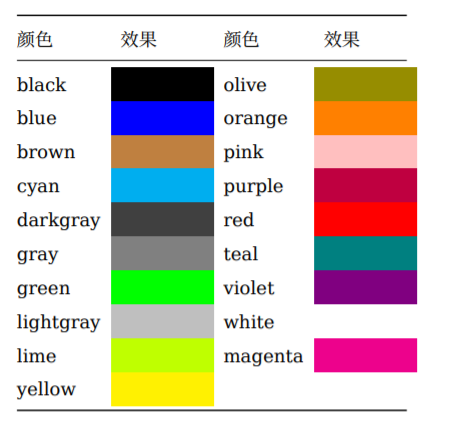
\includegraphics[scale=1 , keepaspectratio]{xcolor.png}
\end{figure}

上面的图片所用的表格Tex代码用到了 \verb+cellcolor+ 这个命令,这在epub那边不能正常显示。这段代码贴出来吧,权做参考。

\begin{Verbatim}
\begin{table}[H]
\centering
\begin{tabular}{@{}lp{50pt}lp{50pt}@{}}
\toprule
颜色        & 效果  & 颜色       & 效果\\ \midrule
black     &  \cellcolor{black}  & olive     &    \cellcolor{olive} \\
blue      &   \cellcolor{blue} & orange    &   \cellcolor{orange}\\
brown     &  \cellcolor{brown}  & pink      &   \cellcolor{pink}\\
cyan      &   \cellcolor{cyan} & purple    &   \cellcolor{purple}\\
darkgray  &  \cellcolor{darkgray} &red       &   \cellcolor{red}  \\
gray      &   \cellcolor{gray} & teal      &    \cellcolor{teal}\\
green     &   \cellcolor{green} & violet    &   \cellcolor{violet}\\
lightgray &  \cellcolor{lightgray} &white     &   \cellcolor{white} \\
lime      &    \cellcolor{lime} & magenta   &   \cellcolor{magenta} \\
yellow    &    \cellcolor{yellow}\\ \bottomrule
\end{tabular}
\caption{直接可以使用的颜色名字}
\label{tab:直接可以使用的颜色名字}
\end{table}
\end{Verbatim}


如果你加载xcolor宏包时填上其他选项,比如svgnames等,就会有更多其他颜色的名字可以直接使用了。具体请参看\href{http://mirrors.ctan.org/macros/latex/contrib/xcolor/xcolor.pdf}{xcolor官方文档}。


\subsection{单个颜色调百分比}
虽然颜色混合我弄不大明白,不过单个颜色调百分比\footnote{不清楚和谁调?白色?}还是很有用的。比如gray灰色后面跟个!20,就表示20\%的灰。请看下面不同百分比的红色。

\begin{Verbatim}
\begin{table}[H]
\centering
\begin{tabular}{@{}lp{50pt}lp{50pt}@{}}
\toprule
颜色        & 效果  & 颜色       & 效果\\ \midrule
red     &  \cellcolor{red}  & red!90     &    \cellcolor{red!90} \\
red!80      &   \cellcolor{red!80} & red!70    &   \cellcolor{red!70}\\
red!60     &  \cellcolor{red!60}  & red!50      &   \cellcolor{red!50}\\
red!40      &   \cellcolor{red!40} & red!30    &   \cellcolor{red!30}\\
red!20  &  \cellcolor{red!20} &red!10       &   \cellcolor{red!10}  \\
red!0    &    \cellcolor{red!0}\\ \bottomrule
\end{tabular}
\label{tab:不同百分比的灰色}
\caption{不同百分比的灰色}
\end{table}
\end{Verbatim}


\begin{figure}[H]
\centering
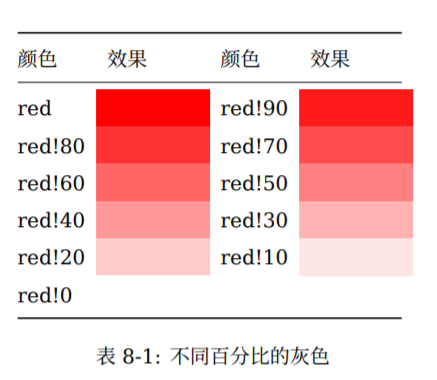
\includegraphics[scale=1 , keepaspectratio]{xcolor_mix.png}
\end{figure}

值得一提的是xcolor宏包还支持一种表格颜色交替模式,看上去不错。请看带颜色的表格这一小节\ref{sec:带颜色的表格}。

\chapter{表格环境}

\section{表格横向一半的线条}
cmidline类似于原来的cline命令,简单来说就是你希望第几个到第几个格子画一条线。这个命令后面一样可以跟个描述粗细的可选项。请看下面的例子:

\begin{Verbatim}
\begin{table}[H]
\centering
\begin{tabular}{@{}lll@{}}
\toprule
slices      & \multicolumn{2}{l}{abs.error(slices)} \\ \cmidrule(l){2-3} 
            & avg.              & max               \\ \midrule
<5000       & 116               & 625               \\
5000-10000  & 209               & 1807              \\
10000-15000 & 297               & 2133              \\
>15000      & 317               & 1609              \\ \bottomrule
\end{tabular}
\caption{cmidrule例子}
\label{tab:cmidrule例子}
\end{table}
\end{Verbatim}

显示效果如下:

\begin{figure}[H]
\centering
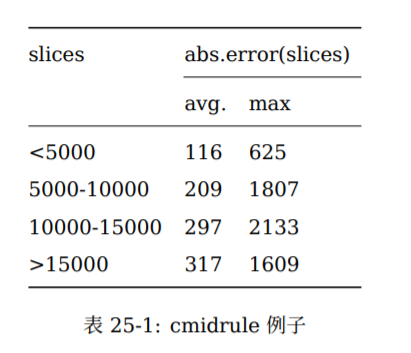
\includegraphics[scale=1 , keepaspectratio]{cmidline.png}
\end{figure}


\section{表格放大或缩小}
用scalebox和resizebox命令除了可以放大或者缩小图片之外,也可以用于放大或者缩小表格,这是值得注意的一件事,因为在排版的时候对表格的大小调整有的时候也是很重要的。

\emph{值得一提的是现在在表格里面verb命令不可以用了,会出错。}

\begin{Verbatim}
\begin{table}[H]
\rowcolors{2}{}{lightgray!50}
\centering
\resizebox{\linewidth}{!}{
\begin{tabular}{@{}ll@{}}
\rowcolor{lightgray!20}
表格放大        &     说明         \\ 
1        & 2           \\
3              & 4             \\
5      &  6        
\end{tabular}
}
\caption{表格放大}
\label{tab:表格放大}
\end{table}
\end{Verbatim}

显示效果如下:

\begin{figure}[H]
\centering
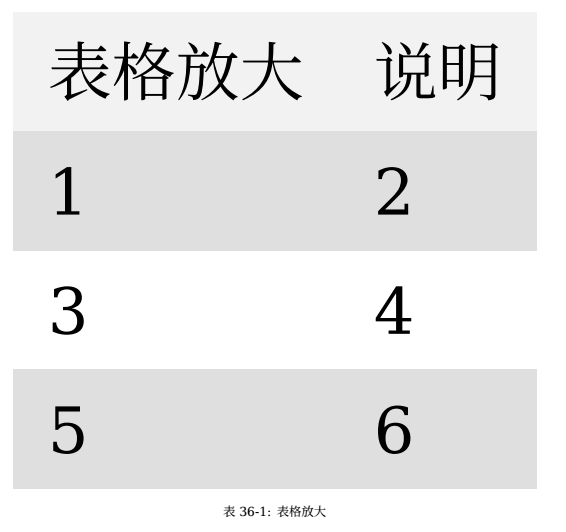
\includegraphics[scale=1 , keepaspectratio]{scale_table.png}
\end{figure}



\section[带颜色的表格]{带颜色的表格\footnote{本小节除了参看wikibook之外还参看了\href{http://texblog.org/tag/definecolor/}{这个网站}。}}
\label{sec:带颜色的表格}
xcolor宏包提供了一种颜色交替的表格模式,还挺好看的。好吧,我对颜色搭配不太擅长。首先需要在加载xcolor宏包时填上table可选项,即:

\begin{Verbatim}
\usepackage[table]{xcolor}
\end{Verbatim}


\begin{Verbatim}
\begin{table}[H]
\rowcolors{2}{}{lightgray!50}
\centering
\resizebox{\linewidth}{!}{
\begin{tabular}{@{}ll@{}}
\rowcolor{lightgray!20}
实现本表步骤        &     备注         \\ 
table环境下加上rowcolors命令        & 让整个表格交替显色           \\
rowscolors第一个选项              & 决定颜色从那一行开始显示              \\
rowscolors第二个选项            & 奇数列的颜色  \\
第三个选项  & 偶数列的颜色 \\
本表具体代码    &   {\small \textbackslash rowcolors\{2\}\{\}\{lightgray!50\}} \\
第一行用rowcolor命令控制       & 在表头行上面           
\end{tabular}
}
\caption{带颜色的表格}
\label{tab:带颜色的表格}
\end{table}
\end{Verbatim}

\begin{figure}[H]
\centering
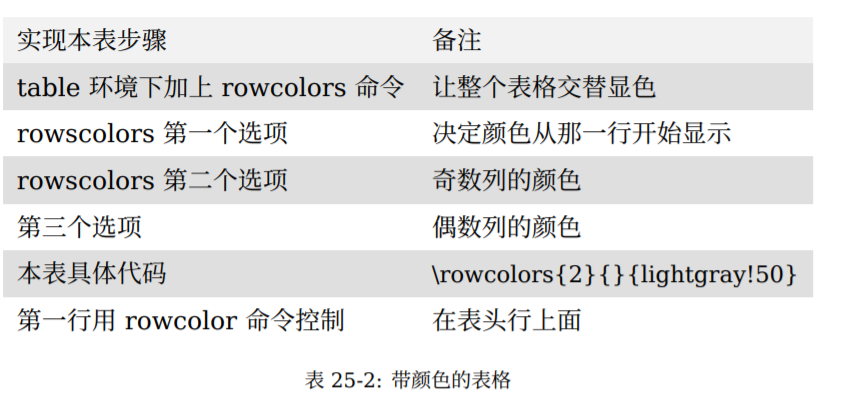
\includegraphics[width=\linewidth ,totalheight=0.95\textheight , keepaspectratio]{color_table.png}
\end{figure}


\chapter{代码环境}
\section{tcolorbox宏包}
这里用tcolorbox宏包的主要是想给代码块就是加上背景颜色。

\begin{Verbatim}
%minted
\RequirePackage{minted}%
\RequirePackage[minted]{tcolorbox}%
\tcbuselibrary{breakable}
\newtcblisting{tcbminted}[2][]{listing engine=minted,
minted style=colorful,minted language=#2,
minted options={fontsize=\footnotesize},
colback=blue!5!white,colframe=blue!75!black,
listing only,#1,breakable=true}

\begin{tcbminted}{python}
class Hero():
    def addlevel(self):
        self.level=self.level+1
        self.hp=self.hp+self.addhp

class Garen(Hero):
    def __init__(self):
        self.level=1
        self.hp=455
        self.addhp=96
        self.skill=['不屈','致命打击','勇气','审判','德玛西亚正义']

garen001=Garen()
for i in range(6):
    print('级别:',garen001.level,'生命值:' ,garen001.hp)
    garen001.addlevel()
print('盖伦的技能有:',"".join([x + '  ' for x in garen001.skill]))
\end{tcbminted}
\end{Verbatim}

\begin{figure}[H]
\centering
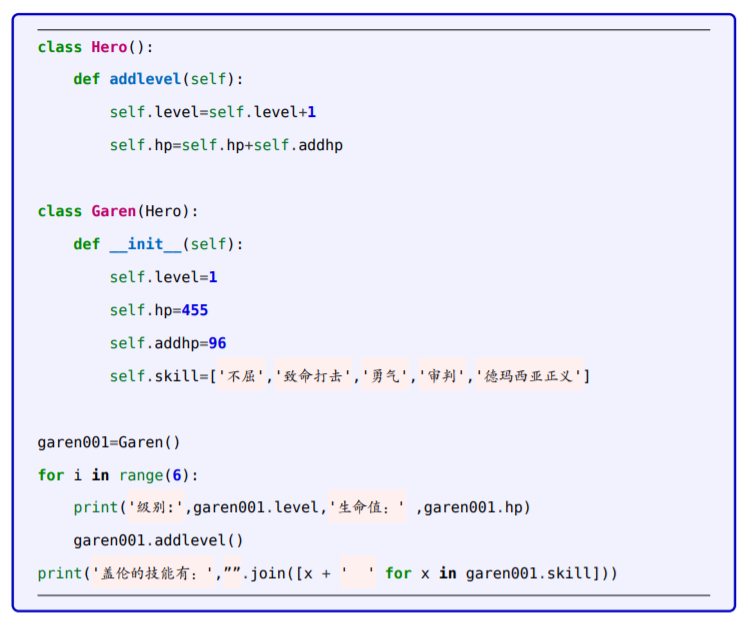
\includegraphics[width=\linewidth ,totalheight=0.95\textheight , keepaspectratio]{tcolorbox.png}
\end{figure}


\chapter{数学环境}
\section{siunitx宏包}
在排版物理书籍的时候常遇到一个问题,那就是比如10cm或者10米等等这样的数字加单位组合我们该如何排,特殊的符号或者一串公式甚至一大串公式当然用数学环境排这是没有疑问的,对于这样短小的数字和单位一般通用的做法是如何的呢?

一般的数字当然就是直接写,然后一般的单位也是直接写,比如10cm啊10米啊就是标准的做法。然后有些特殊的单位符号以及上标下标问题等如果用数学环境写,就会破坏文档这部分内容的谐调性,\emph{siunitx}宏包就是来解决这个问题的。

比如说\verb+\num{3d10}+的显示效果就是 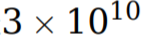
\includegraphics[height=1.2\fontcharht\font`\B ]{siunitx_1.png},比如说\verb+100\si{\text{厘米}^3}+的显示效果就是 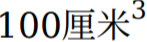
\includegraphics[height=1.2\fontcharht\font`\B ]{siunitx_2.png} 。

值得一提的是原来xeCJK宏包会让数字和中文(单位)之间自动空一格,这很好,而使用了num命令或si命令之后这个自动空格机制被干扰了,你可以选择重新包装这个命令或者手动空一格吧。

siunitx宏包还有一个好处就是对于某些特殊的符号的输入也提供了支持,比如温度的度 \verb+\si{\degreeCelsius}+ 显示效果是 
\includegraphics[height=1.2\fontcharht\font`\B ]{siunitx_3.png} 等等,此外还可以定制一些额外的符号:
\begin{Verbatim}
\sisetup{
math-micro = \text{μ},
text-micro = μ
}
\end{Verbatim}
这样你就可以用\verb+\si{\micro m}+来显示
\includegraphics[height=1.2\fontcharht\font`\B ]{siunitx_4.png}了。当然了这个宏包说白了就是对数学环境下某一些符号命令的text命令的一种包装吧,如果你能够直接输入那个符号就直接输入吧,这就是推荐的做法。

简单说来就是短小的数字或单位等还是不要麻烦数学环境了。更多的内容请参看siunitx官方文档,还可以参看\href{http://tex.stackexchange.com/questions/37168/when-to-use-math-mode}{这个网站}。



\chapter{图片环境}
\section{导入pdf页面}
这里要讲的是使用pdfpages宏包来实现多个pdf页面的导入。\\
\verb+\usepackage[options]{pdfpages} +\\
默认是插入所有pdf页面,还有一些选项请参看文档。最常用的选项就是:\\
\verb+pages={1,{},8-10}+\\
上面的意思是插入第一张页面,然后插入一个空页面,然后插入第八张到第十张。


\section{图片宽度最大宽度设置}
在我学习html的时候发现html里面放置图片很方便设置max-width这个属性,大部分图片的宽度就不用操心了,心想latex可以实现这样的功能吗。就是图片宽度不超过你给定的max-width则图片是原宽度,如果超过了,则将其缩放到最大宽度,这样图片就不超过pdf的有效页面了。后来找到了 \href{http://tex.stackexchange.com/questions/86350/includegraphics-maximum-width}{这个网页} 给出的解决方案,很是不错 。

具体代码如下所示:
\begin{Verbatim}
\includegraphics[keepaspectratio,max width=0.95\linewidth]{images/lena.jpg}
\end{Verbatim}

你需要加载 \textbf{adjustbox} 宏包:
\begin{Verbatim}
\RequirePackage[export]{adjustbox}% 'export' is needed
\end{Verbatim}



\chapter{多栏环境}
\section{multicol宏包}
多栏环境推荐使用\emph{multicol}宏包。\footnote{在beamer类下有一种看上去不错的多栏环境,就是使用的columns环境,不过只适用于beamer类的frame框架下。}
这个宏包很厉害,支持两栏到十栏的环境。就作为通用的一般形式如下:

在这里每一栏的宽度表示为linewidth,这个可以用来控制放进去的图片宽度。
这里用columnbreak命令手动调整栏的跳转。你也可以不用columnbreak命令,而让\TeX 自动计算栏的高度和分布等。不过似乎用columnbreak只能近似控制,并不是那种完全严格的跳转命令。
这是最基本的应用,请参看多张图片并列显示这一小节。\ref{sec:多张图片并列显示}

代码大致是这样的:

\begin{Verbatim}
\begin{multicols}{2}
\setlength{\columnseprule}{0.4pt}
如果你希望整个文档都分为两栏,那么在前面documentclass命令可选项里面加上twocolumn即可。这里的分栏环境是分两栏,然后加入的分栏线。就是在分栏环境中用setlength调整长度量columnseprule为0.4pt\footnote{参考了\href{http://texblog.org/tag/columnseprule/}{这个网站}}。觉得这个命令应该重新修改下,直接\textbackslash columnseprule就是加分栏线,然后后面跟个可选参数表示线的宽度。

还有一个长度量columnsep表示栏之间的间距宽度,一样用setlength调节。一般没啥好调整的。分栏环境就这样简单说下吧。
\end{multicols}
\end{Verbatim}


\begin{figure}[H]
\centering

\includegraphics[width=\linewidth ,totalheight=0.95\textheight , keepaspectratio]{multicolumn.png}
\end{figure}


\section{分栏环境备用}
在实际应用过程中,常常遇到分两栏的情况,但是这两栏宽度是可以自由调整的。我找了一下似乎并没有类似beamer类columns环境那样方便的存在,只好通过minipage命令简单地实现了类似的效果。实际应用我是通过texmaker自定义快捷输入代码模块功能快速输入进文档的。
\begin{Verbatim}
\noindent
\begin{minipage}{\textwidth}
\begin{minipage}{0.3\textwidth}
\begin{table}[H]
\centering
\medskip 
\scalebox{0.82}{
\begin{tabular}{@{}ll@{}}
\toprule
$t$(分) & $s$(英尺)  \\ \midrule
0 & 0     \\
1 & 1200  \\
2 & 4000  \\
3 & 9000  \\
4 & 9500  \\
5 & 9600  \\
6 & 13000 \\
7 & 18000 \\
8 & 23500 \\
9 & 24000 
\\ \bottomrule
\end{tabular}
}
\caption*{表 2-1}
\end{table}

\end{minipage}\hfill
\begin{minipage}{0.7\textwidth}

\begin{figure}[H]
\centering
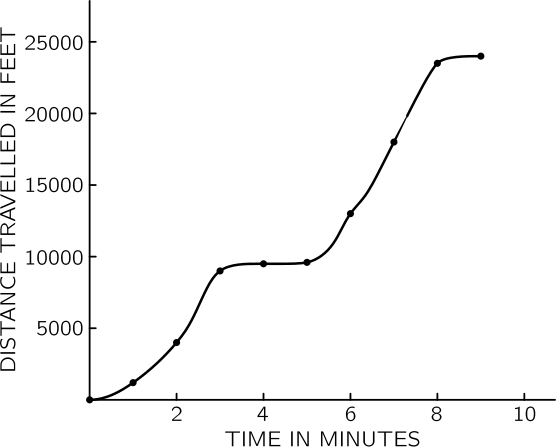
\includegraphics[width=\linewidth ,totalheight=0.95\textheight , keepaspectratio]{ju-li-shi-jian-qu-xian-tu.png}
\caption{汽车的距离-时间曲线}
\label{fig:ju-li-shi-jian-qu-xian-tu}
\end{figure}

\end{minipage} 
\end{minipage} 
\end{Verbatim}

最后显示效果如下:

\begin{figure}[H]
\centering
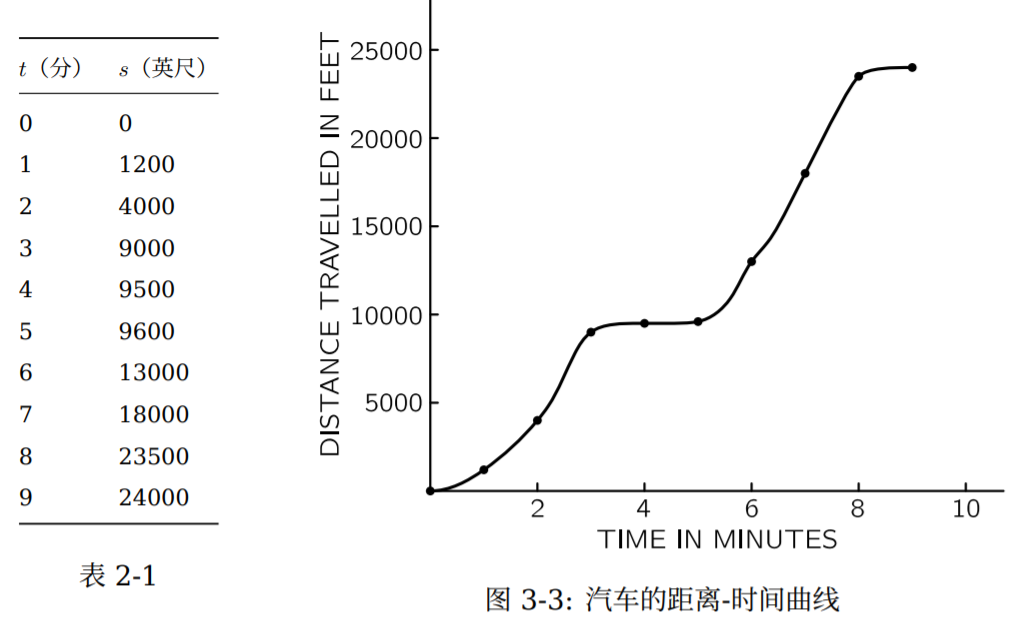
\includegraphics[width=\linewidth ,totalheight=0.95\textheight , keepaspectratio]{multicolumn_2.png}
\end{figure}





\chapter{如何显示更多的特殊符号}
本小节内容建议读者从理解Tex字体的原理来学习,但真的不推荐使用。

现在让我们将思路先理清一下。首先是Unicode码,这个只是一个理论上的编码规则,具体的实现是字体。但是每一个字体都只专注于某一个领域,并没有把Unicode所有的码都画出字形来,那么系统是如何显示字体的呢?系统是安装了很多字体,如果一个字体并不包含它要显示的Unicode,它就搜索打开下一个字体文件,找相关的Unicode的字形。只有从字体文件中具体找了这个Unicode的字形,才有办法将其显示出来。
\footnote{主要参考了\href{http://tex.stackexchange.com/questions/41130/getting-xelatex-to-display-accents-and-characters-not-included-with-the-font}{这个网站}}

现在我希望显示Ubuntu的那个图标,那个图标实际上也是一个字体。具体配置代码如下:

\begin{Verbatim}
\newfontfamily{\ubuntu}[Scale=2]{Ubuntu}
\usepackage{newunicodechar}
\newunicodechar{}{{\ubuntu{}}}
\end{Verbatim}

主要是利用的newunicodechar宏包。这个宏包就只有一个命令,这个命令就是这个宏包的名字。其实我们能够猜到,这个命令的作用就是将这个字符变成类似\TeX 命令的东西,然后替换为后面的那一串,而后面的那一串单独提出来也是能够正常显示的。具体效果就是这个Ubuntu图标你直接在Tex文档上复制粘贴到哪里了,就能够显示。甚至你的操作系统都没办法显示出来只是一段空白。

\begin{figure}[H]
\centering

\includegraphics[scale=1 , keepaspectratio]{ubuntu_logo_font.png}
\end{figure}

这里有一段代码生成该字体所有已有的字形\ref{sec:字体已有字形}。当然你可以直接在字符映射表里面选择只显示已有字形查看,不过有时并不方便。生成那个pdf查看之后可以复制粘贴,到那个字符映射表里面搜索,还是很方便的。



\chapter{旁注}
\LaTeX 自带的有marginpar命令就是插入旁注的(你需要把页面布局的旁注部分设置好。)我也接触过另外一个宏包的marginnote命令,虽然多了一个可选项可以调整旁注竖向位移,但是带来的麻烦更多,有时候页尾的旁注会向下越界,如果我想写了一个旁注,又在下面继续写一个旁注命令也会出现重叠出错。而marginpar就没有这样的问题。写了一个marginpar,后面可以继续再开一条marginpar命令。至于竖向位移的问题,使用vspace命令调整即可。

下面是我新建的一个rightnote命令,以供参考。
\begin{Verbatim}
\newcommand{\rightnote}[1]{\marginpar{  
 	\fontsize{10pt}{12pt}\selectfont #1}}
\end{Verbatim}

在maginpar命令里面进行各种\LaTeX 命令都是可以的,比如改变字体大小,字体颜色,插入图片等等。



\chapter{尾注}
\textbf{NOTICE:} 本文档已经取消了endnotes功能,也不推荐读者使用,一切从简,脚注其实已经很好地满足需求了。下面本章的内容更多的可以用来作为参考来学习Tex内部机制和如何编写latex宏包。

尾注也就是每一章后面的注释部分,这种排版形式显得更加专业。而且如果尾注写的好参考文献一章或者其他附录部分都可以不用写了。

本来已经有一个endnotes宏包了,但是这个宏包不支持超链接,然后后来我按照\href{http://tex.stackexchange.com/questions/8452/making-endnotes-clickable-links-with-hyperref}{这个网站}的说明操作加入另外一个sty文件之后是能够正常双向链接的,但是为了解决一个问题引入两个宏包,而且这两个宏包还存在交互问题只是让问题更加复杂了。

我试着慢慢将这两个宏包融合起来,遇到了很多困难,因为我对tex原初命令并不是十分熟悉,最终似乎解决了这一问题。其中有些细节我也不大清楚,下面就这个新的endnotes宏包详细说明。


\section{endnotes宏包说明}
整个宏包还是很简洁的,满打满算八九十行。宏包的文件在github源码的texmf文件夹里面。


\begin{Verbatim}
\NeedsTeXFormat{LaTeX2e}[1994/12/01]
\ProvidesPackage{endnotes}[2013/11/29 v0.12  endnotes]
\end{Verbatim}
首先是一些文档的注释说明信息,这里就不写了。

然后是标准的宏包sty文件的开头样式,这里填上endnotes宏包即可。

\begin{Verbatim}
\RequirePackage{etoolbox}
\DeclareRobustCommand*{\flabel}[2]%
{\phantomsection \def\@currentlabel{#2}
\label{#1}}%
\end{Verbatim}

这里使用RequirePackage命令引入了etoolbox宏包,主要是为了引入了expandonce命令,这个命令是确保后面的一个命令只运行一次。

然后接下来新建了一个命令flabel,这个命令是为了文本中的尾注标记符号和尾注中的标记符号区分开来,比如文本中的尾注标记符号是上标的,而尾注中的标记符号则不是。flabel命令里面使用了hyperref宏包的精确定位命令phantomsection,因为hyperref宏包在myconfig宏包中已经加载了,这里就不加载了。

flabel命令接受两个参数,第一个参数\#{}1表示真实的label,而第二个参数\#{}2表示显示的label。所谓真实的label指等下生成的pdf中的精确定位label标记。命令中重新定义了\verb+\@currentlabel+,也就是显示的label。这样将这两者区分开来,本来他们都是一样的。



\begin{Verbatim}
\gdef\theenmark{\arabic{@EndnoteCounter}}%
\gdef\endnotemark{\textsuperscript{(\theenmark)}}%
\gdef\endnotemarkback{(\theenmark)}%
\end{Verbatim}
然后上面三行定义了一些对外的接口命令,方便DIY。theenmark命令是尾注标记符号的计数器部分,这里使用了arabic命令转化了。endnotemark命令是文本中尾注标记符号的形式,这里简单加上了()然后使用textsuperscript命令将其转化成为上标形式,之所以使用这样的形式,是因为使用数字可以没有任何限制,而使用其他奇怪的符号标记要为可能超过界限操心。而endnotemarkback命令则是尾注中的标记符号形式,这里和前面的区别就是没有转化成为上标。

\begin{Verbatim}
\newlength{\enoteindent}
\setlength{\enoteindent}{2.5\textpt}
\end{Verbatim}
这段代码的意思是设置了一个长度量enoteindent,然后将其设置为2.5倍textpt长,这个textpt之前说过的是为了让文档相对化将之前documentclass设置的12pt传递过来的,你也可以在这里设置成一个你喜欢的长度。这个长度影响等下尾注标签的缩进量。


接下来下面的代码首先用newwrite命令新建了文件,tex中的文件操作命令如下:
\begin{Verbatim}
\newwrite\tempfile
\immediate\openout\tempfile=lists.txt
\immediate\write\tempfile{this is test}
\immediate\closeout\tempfile
\end{Verbatim}
这里的newwrite是新建一个写文件,然后后面immediate命令表示立即执行,openout表示打开某个文件,这里打开了新建的这个写文件\textbackslash tempfile,后面的等号跟着你想要的这个新文件的文件名,等下电脑中新建出来的这个文件就是这个文件名。

然后write命令是往这个文件里面写入某个文本信息。接下来是closeout命令把这个文件关闭,只有文件正常关闭了写的内容才能从缓冲区真正进入系统中的文本。


\begin{Verbatim}
\newwrite\@entout

\newcounter{@EndnoteCounter}%
\newcounter{@AllEndnoteCounter}%
\newcounter{@ShowEndnoteCounter}%
\setcounter{@EndnoteCounter}{0}
\setcounter{@AllEndnoteCounter}{0}
\setcounter{@ShowEndnoteCounter}{1}

\newif\if@entopen \global\@entopenfalse
\end{Verbatim}
接下来是新建了三个计数器@EndnoteCounter等,其中@EndnoteCounter标记每一章尾注内部的计数,而AllEndnoteCounter标记了所有的尾注的计数,这个影响真实label。ShowEndnoteCounter标记了每一个分章的章数(这里主要指按照每一章,不过实际操作并不局限于此。)的计数。然后用setcounter命令给这些计数器一个初值。

上一段代码最后还新建了一个条件控制变量,具体请参看tex条件控制语句一小节\ref{sec:条件控制语句}。这里的global命令是让接下来的定义或者声明是全局性的。

\begin{Verbatim}
\def\@openent{%
\def\@entname{\jobname
\ifnum\value{@ShowEndnoteCounter}<10 0\fi
\ifnum\value{@ShowEndnoteCounter}<100 0\fi
\arabic{@ShowEndnoteCounter}}%

\immediate\openout\@entout=\@entname.ent%
\global\@entopentrue
}%
\end{Verbatim}
上一段代码新建了一个命令@openent,这个命令等下要完成打开新建的ent文件任务,然后正如前面谈及的文件操作,在openout命令打开文件的时候,这里对具体生成的ent文件的文件名进行了一些DIY。其实我可以将文件名简单设置成为jobname-1,-2之类的形式,之所以弄成以上这种形式多少是我在之前探索过程中弄出的一种jobname001,jobname002这种形式,然后方便使用linux系统的cat命令来将他们汇总,后来修改修改着这个功能发现不需要了,但这个技巧还是很有用的就没删除了。

下一段的解释先跳过,看到下下一段定义的endnote命令。
\begin{Verbatim}
\begingroup \catcode `|=0 \catcode `[=1
\catcode`]=2 \catcode `\{=12 \catcode `\}=12
\catcode`\\=12
|gdef|@writeent[|immediate|write|@entout[
{\footnotesize
\hspace{-2\parindent}\makebox[\parindent-3pt][l]
{\flabel{|@linknameb}{|@showlinknameb}  \ref{|@linkname}}
\leftskip=\parindent   |expandonce|@include \par } ] ]%
|endgroup
\end{Verbatim}
上面这段代码就是定义了那个@writeent,但是以一种十分绕脑袋的形式,我也没完全弄明白。。首先看到catcode命令,这个是改变tex系统内部字符列表的命令。在tex中字符分为以下几类:
\begin{enumerate}
\setcounter{enumi}{-1}
\item 跳脱符号,一般是\textbackslash
\item group开始符号,一般是\{
\item group结束符号,一般是\}
\item 数学符号,一般是\$
\item 表格分隔符,一般是\&
\item 一行结束符号,一般是<return>
\item 参数符号,一般是\#
\item 上标符号,一般是\^{}
\item 下标符号,一般是\_
\item 忽略符号,一般是<null>
\item space,一般是<space>和<tab>
\item 字母,一般是a-z和A-Z
\item 其他,不是其他分类就在此类
\item 激活(Active)符号,比如\~{}
\item 注释符号,一般是\%
\item 无效(Invalid)符号,一般是<delete>
\end{enumerate}
也就是说tex引擎看到\textbackslash 符号就会认为接下来将是一个命令,然后catcode命令可以改变这个列表。比如上面这段代码中,\verb+\catcode `|=0+就将|符号归为0类,这样tex看到|也会跟看到\textbackslash 一样处理。后面的类似,于是我们有:\\
\emph{|类似\textbackslash{  }   [类似\{  ]类似\}  \{\} \textbackslash 都是其他 }

gdef命令是global和def命令的组合缩写,这里定义了下面要用到的@writeent命令。就是立即向打开的那个ent文件写入花括号内的信息。其中的符号变化法则上面谈及了,于是这里的\textbackslash footnote之类的都不会处理,而是直接写入ent文件之中。但是因为我们在这里要建立label(等下插入ent文件之后,在尾注那里要标记label和ref命令。)因此label和ref内的参数必须立即运算出来。在这里有一些尾注的格式美化命令,比如用makebox命令调整尾注标记符号格式等,这里介绍略过。

现在主要看到从下一段代码中定义的@include命令接受的是endnote命令传递过来的文本,本来在下一段代码中新建一个group然后用let命令将endnote命令中所有的protect命令改成了string(字符串),应该是可以了。实际上操作中确实各个命令没有展开直接以文本进入ent文件了,但是环境命令还是展开了,于是这里加上了etoolbox宏包提供的expandonce命令,也就是控制只展开一次,这样环境命令也成功传递过去了。这里的具体实现细节我实际上也没弄太明白。

\begin{Verbatim}
\DeclareRobustCommand*\endnote[1]{%
\stepcounter{@EndnoteCounter}%
\stepcounter{@AllEndnoteCounter}%
\edef\@linkname{enote:\arabic{@AllEndnoteCounter}}%
\edef\@linknameb{enote:\arabic{@AllEndnoteCounter}b}%
\edef\@showlinknameb{\endnotemark}%
\edef\@showlinkname{\endnotemarkback}%
\ignorespaces\flabel{\@linkname}{\@showlinkname}%
\ignorespaces\hspace{-0.5ex}\ref{\@linkname b}%
\if@entopen \else \@openent \fi%
\begingroup%
\let\protect\string%
\gdef\@include{#1}%
\endgroup%
\@writeent%
}
\end{Verbatim}
显然你看到这里定义的命令endnote就知道这是这个宏包的主体部分,程序一般遇到的就是两个命令,endnote引入尾注,showendnotes插入尾注。首先这个命令将两个主要计数器加1,其中@EndnoteCounter计数器是标记一章尾注内部的计数的,这里加1了就开始从1开始,然后后面这里的处理技巧是如果你需要插入尾注了,那么就将@EndnoteCounter这个计数器归为零。这样做和将@EndnoteCounter和chapter或者part绑定起来的好处就是更加的自由,你不需要考虑什么,甚至在某一个section部分内,插入showendnotes命令就插入了尾注,然后内部计数又重新开始。

接下来定义了四个命令,我们看到这里有一个edef命令,edef命令和def命令类似,区别在于定义某个命令的时候立即展开,比如在这里我edef了一个@linkname命令,那么后面的@AllEndnoteCounter当时是什么立即赋值计算出来。因为这里要建立label的名字比如是独一无二的,然后看到后面@showlinkname和@showlinknameb,这是在决定文档中尾注标记符号和尾注中标记符号的样式,这里名字弄翻了,因为之前我在编写的时候也不大确切,然后后面就交换了一下。

然后我们注意到这个endnote命令后面每一行都有一个\%,这是不得已而为之。endnote命令在它所在地地方我需要插入label和ref,然后每一行换行之后都会增加一个空格。只好用百分号消去。

这里插入的ignorespaces命令为了消去空格可能是多余的,然后使用flabel命令植入label,前面谈及了第一个参数是真实的label,第二个参数是显示的label。还有我们需要把label命令和ref命令的关系弄清楚,label只是在文档中植入一个记号,而ref命令才会在文档中显示某些字符。我在测试的时候发现尾注标签上标记号有点偏后,然后用hspace命令稍作调整,注意我们调整距离尽可能使用ex或者em这样的相对距离。然后就是使用ref命令。

接下来一行语句的意思就是ent那个文件打开了吗?打开了什么也不做,没打开打开这个文件,使用之前定义的openent命令打开。

然后我们进入一个group,tex命令中\textbackslash begingroup \textbackslash endgroup之间夹著一个内环境。这个内环境的作用就是为了把endnote命令中的文本内容传递出去,为什么要这么做?我们的思路是将endnote中的文本写入到某个ent文件中去,然后继续写,直到要插入尾注了再引入这个ent文件即可。思路很简单,但是要实现起来并不简单。

这里最大的问题是endnote命令里面的命令和环境都要不执行,当作文本一行写入进去。因为tex默认参数都要执行计算出来的,这就是问题的所在。这里面的细节甚是复杂,我也没完全弄明白。我们再看到上面那段代码定义的@writeent命令。


\begin{Verbatim}
\DeclareRobustCommand*\showendnotes{%
\immediate\closeout\@entout%
\global\@entopenfalse

\input{\@entname.ent}

\setcounter{@EndnoteCounter}{0}
\stepcounter{@ShowEndnoteCounter}%

}

\endinput
\end{Verbatim}
这是宏包的最后一段了,非常容易理解了。定义了一个showendnotes命令,命令首先将那个打开的ent文件关闭,这样之前写入的内容都写进去了。然后改变那个条件变量表明文件关闭了。然后引入尾注。
然后@EndnoteCounter计数器归零,这个前面谈到过。然后ShowEndnoteCounter计数器加一。然后结束宏包使用endinput命令。


\section{endnotes宏包的使用}
在加载好endnotes宏包之后,用法还是很简单的。

\subsection{endnote命令}
想要在那里插入尾注部分注释就用endnote命令即可:\\
\verb+\endnote{这是一段尾注}+。比如这里\footnote{这是一段尾注}。

\subsection{showendnotes命令}
在你想要显示尾注时,使用showendnotes命令即可。那么到目前为止,所有尾注内容都会显示出来:\\
\verb+\showendnotes+

一般上面还加上一个标题,表示注释内容就在这里。如果整个文档都不使用showendnotes命令,那么也不会有什么错误。





\part{xelatex高级篇}
本部分关注于tex最底层的一些概念和原理,有些知识点了解之后对读者如何定制latex原有的命令和功能有所帮助,有些能够加深读者对tex底层如何工作的理解。

\chapter{长度量}
\section{单位}
\LaTeX{}中常见的长度单位如下表所示:
\begin{table}[H]
\centering
\caption{\LaTeX{}中的常见长度单位}
\label{tab:LaTeX中的常见长度单位}
\medskip 
\begin{tabular}{@{}lll@{}}
\toprule
单位 & 说明 & 换算法则 \\ \midrule
pt  &   &\\
mm  & 一毫米  & 1mm=2.84pt \\
cm  &  一厘米  &  1cm=28.4pt \\
in  &  一英寸 & 1in=72.27pt \\
ex  &  (相对长度)大约相当于当时字体的x高度 & \\
em  & (相对长度)大约相当于当时字体的M宽度 & \\ \bottomrule
\end{tabular}
\end{table}


\section{默认的长度量}
\begin{itemize}
\item \textbf{\textbackslash evensidemargin ~ \textbackslash linewidth ~ \textbackslash oddsidemargin ~ \textbackslash paperwidth ~  \textbackslash paperheight ~ \textbackslash textheight ~ \textbackslash textwidth ~ \textbackslash topmargin }:这些长度量都和页面布局有关,很多都在前面页面布局那一节里面说了,这里就不赘述了。
\item \textbf{\textbackslash baselineskip ~ \textbackslash baselinestretch ~\\ \textbackslash baselineskip ~  \textbackslash parindent  ~ \textbackslash parskip }:这些长度量和段落格式有关,大多都在前面段落一节说了,这里也不赘述了。
\item \textbf{\textbackslash columnsep ~ \textbackslash columnwidth ~ \textbackslash tabcolsep ~ \textbackslash unitlength}:这几个长度量和特殊的环境有关,比如columnsep控制多栏环境之间的宽度,columnwidth控制栏的宽度,tabcolsep控制tabular环境一列一列之间的间距,unitlength控制picture环境下的unit的长度(还不太清楚)。
\end{itemize}

 
\section{定义自己的长度量}
要新建一个自己的长度量使用newlength命令即可:\\
\verb+\newlength{\lengthname}+

\section{修改长度量}
用setlength命令直接设值某个长度量的值为多少。\\
\verb+\setlength{\lengthname}{20pt}+

此外还可以使用addtolength命令来给某个长度值加上一个数值。\\
\verb+\addtolength{\lengthname}{20pt}+

\section{使用长度量}
长度量一般在该使用的地方可以直接使用,其中伸缩量可以跟一个plus量和一个minus量。此外长度量还支持前面加个实数表示相乘多少的形式。\\
\verb+0.7\lengthname+

\subsection{显示长度量的值}
要在pdf文档中显示某个长度量的值使用\textbackslash the命令即可:\\
\verb+\the\lengthname+

\section{calc宏包介绍}
前面提及的setlength,addtolength命令只能接受最简单的长度量,在引入calc宏包之后可以进行一般的中缀数学表达式的运算。更多内容请读者自己翻看\href{http://mirrors.ctan.org/macros/latex/required/tools/calc.pdf}{官方手册}。




\chapter{计数器}
计数器(counter)之前也接触过一些了,现在基于wikibook和\href{http://texblog.org/2007/07/25/counters-in-latex/}{这篇博文}做一些整理工作。


\section{latex默认的计数器}
\begin{itemize}
\item \textbf{part chapter section subsection subsubsection paragraph \linebreak subparagraph} 这些计数器我们在前面的章节编号形式修改那一小节中有所接触,具体请参看章节编号形式修改这一小节:\ref{sec:章节编号形式修改}。
\item \textbf{equation figure table} 这三个是浮动体环境的计数器,其中figure我们在前面的图片标题的修改那一小节有所接触,具体请参看图片标题的修改这一小节:\ref{sec:图片标签的修改}。
\item \textbf{page footnote mpfootnote} page看得出来是页面的计数器,还没怎么接触。footnote是脚注的计数器,这个在DIY脚注的时候会接触到,mpfootnote是minipage下的脚注的计数器,这个知识点参看的\href{http://tex.stackexchange.com/questions/18499/how-to-change-symbol-for-footnote-in-minipage}{这个网站}。
\item 此外enumerate环境里面还有专门的计数器:\textbf{enumi enumii enumiii enumiv}。enumi记录的是当前enumerate环境第一级的item出现的次数,后面的依次是第二级第三级等等,不怎么常用。具体请参看enumerate环境标签的修改这一小节:\ref{sec:enumerate环境标签的修改}
\end{itemize}



\section{使用计数器}
计数器并不可以直接使用,需要使用以下命令来获得某个特殊形式的值。
\begin{description}
\item[value] 将计数器转化为数值方便后面的计算,不能作为字符直接显示。
\item[arabic] 将计数器转化为1 2 3...的形式,可以直接显示。
\item[alph] 将计数器转化为a b c...的形式,可以直接显示。
\item[Alph] 将计数器转化为A B C...的形式,可以直接显示。
\item[roman] 将计数器转化为ⅰ ⅱ ⅲ... 的形式,可以直接显示。
\item[Roman] 将计数器转化为Ⅰ Ⅱ Ⅲ...的形式,可以直接显示。
\item[fnsymbol] 将计数器转化为一系列的特殊符号。
\end{description}

\section{计数器变成带圈的数字系列}
我想新建一个命令,这个命令可以把计数器转化为①②③...这样的形式,可以直接显示。可以看得出来这个命令会很实用的。

\subsection{用tikz画的方法}
\begin{Verbatim}
\newcommand*\circled[1]{%
  \tikz[baseline=(char.base)]\node
  [shape=circle,draw,inner sep=1pt,minimum size=8pt] (char) {#1};}
\newcommand*\circledarabic[1]{\circled{\arabic{#1}}}
\end{Verbatim}

上面这段代码参考了\href{http://tex.stackexchange.com/questions/133264/circled-footnote-symbols-with-pifont-showing-arrows-instead-of-circled-numbers}{这个网站}。看得出来代码大体过程就是利用tikz宏包画出那个符号出来。

这个方法的好处是自由度比较高,根据circled命令,类似的可以定义circledalph——圈圈里面带个字母等。这个方法还有一个好处,虽然①②这样的符号Unicode里面有,但是字体没有,如前面所述,还是需要写上一连串的代码,多少有点费事,而且到后面数字大了总会没有这个字体符号了,就会出错,而这个方法可以避免这些麻烦。推荐使用这个方法。


\section{定义自己的计数器}
用newcounter命令来定义自己新的计数器。\\
\verb+\newcounter{countername}+

\section{修改计数器的值}
系统默认的计数器都是默认设置初始值为0,如果你需要使用这个计数器,首先加一,然后使用这个计数器。
\subsection{计数器设值}
直接将计数器设为某个值用setcounter命令。\\
\verb+\setcounter{countername}{number}+
\subsection{计数器加一}
将计数器数值加一使用stepcounter命令。\\
\verb+\stepcounter{countername}+

\subsection{计数器加多少}
将计数器加上一个数值使用addtocounter命令。\\
\verb+\addtocounter{countername}{number}+

\section{计数器和其他计数器绑定}
在使用newcounter命令定义新的计数器的时候可以后面跟个可选项,可选项里填著另外一个计数器的名字,每当这个计数器加一的时候你定义的新的计数器就会归为零。具体格式如下:
\begin{Verbatim}
\newcounter{mycounter}[chapter]
\end{Verbatim}
这样每当chapter加一也就是到了新的一章,你定义的mycounter将会重新归零。





\chapter{新的命令或环境}
\section{新的命令}
新建命令一般就用newcommand命令\\
\verb+\newcommand{name}[num]{definition}+\\
用法都差不多,第一个必填选项是新建命令的名字,一般前面都加一个\textbackslash 符号。第二个可选选项是新建的这个命令接受的参数,比如你填一个2,那么表示这个命令接受两个参数,在后面definition中引用的时候\#{}1表示第一个参数,\#{}2表示第二个参数。

然后还有这种形式:\\
\verb+\newcommand{name}[num][default]{definition}+\\
多的那个default参数是可选参数的默认值,在definition那边对应的就是 \#{}1。这个可选参数如果不填那么默认值为 \verb+def+ ,然后后面利用这个新的命令可以如下填上那个可选参数。

\begin{minted}{tex}
\newcommand\GoodBye[1][\bfseries]{{#1 Good Bye}}

\GoodBye
\GoodBye[\color{red}]
\end{minted}



下面是具体运行效果:

\begin{figure}[H]
\centering

\includegraphics[scale=1 , keepaspectratio]{self_define_command_1.png}
\end{figure}

\LaTeX 的newcommand命令是由原\TeX 的def命令(还有edef gdef xdef 这里先不管。)而来的。作用原理有点类似于替换展开的功能。比如:\\
\verb+\newcommand{\test}{this is a test line}+\\
你定义了这个test命令,然后后面你输入\textbackslash test,系统遇到\textbackslash test之后就会进行替换操作,就成了后面的this is a test line了。理论上只是简单的文本替换,后面可是跟上随意的命令参数或者环境。不过这只是理论上,实际编写宏包命令的时候会遇到很多复杂的问题,主要是expand展开的控制。

还有一个命令providecommand和newcommand差不多的,区别就是providecommand只是提供命令,如果这个命令已经定义了它就什么都不做。而def一定是完全不动声响的覆盖了。

在编写宏包文件的时候推荐使用DeclareRobustCommand命令,但是有些任务似乎只有def或者edef才能完成,这个我也没弄明白。

\subsection{自定义命令样例}
下面是来自ulem的reduline的原实现代码:

\begin{Verbatim}
\newcommand\reduline{\bgroup\markoverwith
    {\textcolor{red}{\rule[-0.5ex]{1em}{0.4pt}}}
    \ULon}
\end{Verbatim}

为了好玩类似的我还用tikz画了一个小三角形和一个小圆,如果各位看官有更喜欢的标记用于文字强调,类似的用tikz画就是了:

\begin{Verbatim}
\newcommand\utriangle{\bgroup\markoverwith
    {\raisebox{-0.4em}{\makebox[1em][c]{\tikz[blue]
    {\draw(0,0) -- (0.1,0) -- (0.05,0.05) --cycle;}}}}
    \ULon}

\newcommand\ucircle{\bgroup\markoverwith
    {\raisebox{-0.6em}{\makebox[1em][c]{\tikz[red]
    {\draw(0,0) circle  (0.05) ;}}}}
    \ULon}
\end{Verbatim}



\section{新的环境}
\label{sec:新的环境}
新建环境命令格式如下:\\
\verb+\newenvironment{name}[num]{before}{after}+\\
和newcommand命令其他用法都差不多,区别就在于后面有两个宏替换。这里值得一提的是原\TeX 并没有新建环境这个命令,而是\LaTeX 新加进去的。

我们假设我们要新建env这个环境,那么\LaTeX 的工作流程是,创建了两个命令,一个是\verb+\begin{env}+命令;一个是\verb+\endenv+命令。所以简单的来看newenvironment命令就是把它看作开辟了一个group(原\TeX 里面的概念),然后首先执行了before中的命令,然后是环境中的内容,然后是after中的命令,然后退出环境。

这里只是说明一下newenvironment命令的工作原理,具体我们新建环境还是用\LaTeX 的风格,即用newenironment命令,只有在不得已的情况下(通常很复杂的情况)才考虑用\TeX 里面的group概念,那个时候估计是要使用catcode命令。



\subsection{notecard环境}
这个环境编写主要参考\href{http://tex.stackexchange.com/questions/127612/color-text-and-bg-of-verbatim-without-affecting-fancyvrb-line-numbers}{这个网站}。

有一类信息,这类信息和正文关系不太大,但是又很重要适合放在正文中而不是尾注或者脚注中。这类信息需要放在文档右边好不引起人们的注意或者好引起人们的注意。文档中的异常元素通常都有这个效果,在于读者的选择。

notecard环境,一种卡片式记忆环境,长高推荐按照黄金比例来。推荐的颜色有:black olive blue orange brown pink cyan purple darkgray red gray teal green violet lightgray white lime magenta yellow 建议都调淡30。不过推荐一个文档内部一种类型只使用一种颜色,颜色太杂也是不好的。

具体实现代码如下:
\begin{Verbatim}
\newsavebox{\tempbox}
\newenvironment{notecard}[2][white]
 {\noindent\ignorespaces%
 \setlength{\fboxsep}{10pt}
  \newcommand{\tempcolor}{#1}
  \begin{lrbox}{\tempbox}%
  \begin{minipage}{#2}
        \setlength{\parindent}{0pt}
        \setlength{\parskip}{1.618ex}   %段落間距
}
 {
 \ignorespacesafterend%
  \end{minipage}%
  \end{lrbox}%
  \colorbox{\tempcolor}{\usebox{\tempbox}}}
\end{Verbatim}

这个notecard代码环境有点小复杂,主要涉及到\LaTeX 盒子相关高级知识,这里先跳过去,后面会提及再慢慢讲。



\begin{Verbatim}
\begin{flushright}
\begin{notecard}[blue!30]{14em}
不懂Unix的人注定最终还要重复发明一个蹩脚的Unix。

Usenet 签名,1987年11月

{\hfill —Henry Spencer}
\end{notecard}
\end{flushright}
\end{Verbatim}

下面是演示效果:

\begin{figure}[H]
\centering

\includegraphics[width=\linewidth ,totalheight=0.95\textheight , keepaspectratio]{notecard.png}
\end{figure}


\chapter{盒子和glue}
\label{sec:盒子和glue}
\begin{flushright}
\begin{framed}
这里参考了Knuth的The Texbook,但是我并没有将其写入参考文献,因为只是觉得关于box和glue的概念最好参考原初定义,但是并不推荐读者阅读这本书,现在已经是\LaTeX 时代了,不推荐读者使用原始的\TeX 命令,一是不太实用,二是兼容性可能不太好。除非你是宏包编写者,但就作为一般的使用者真的没有必要接触那些原始命令了。还参考了\cite{boxes}
\end{framed}
\end{flushright}

在这里box翻译为盒子没什么问题,就是这个glue翻译为胶水或者橡皮都让我不太满意。在后面我都使用的术语是距离或者间距或者干脆用英文glue。从某种意义上讲glue的直译确实应该译为胶或者胶水,不过觉得距离这个词汇更能够让人们有感觉些:\TeX 排版就是不同的盒子编写和彼此之间距离的设置问题。

\section{基本知识}
最小的盒子就是基于Unicode的字符,这些字符然后组成更大的盒子──单词,然后单词组成更大的盒子──行等等。行是一个盒子,段落也是一个盒子,图片是一个盒子,表格也是一个盒子。而这些盒子按照Knuth的描述都是用glue胶水粘合起来的,或者我们称之为这些盒子之间都存在着空间胶合层。下面就是一个盒子的详细参数:

\begin{figure}[H]
\centering
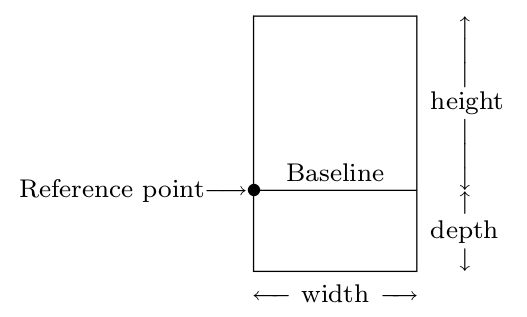
\includegraphics[width=0.8\linewidth ,totalheight=0.95\textheight , keepaspectratio]{box-parameters.png}
\caption{box参数}
\label{fig:box参数}
\end{figure}


盒子就是这么一个长方形的区域,如上图所示,它有参数:height,width,depth。baseline和reference point在后面讲的hbox和vbox中会用到。在\TeX 看来,从字体而来的Unicode 字符就是一个最简单的盒子。字体的设计者已经决定了这个字符的高度,宽度和深度以及它在这个盒子里面看起来如何。\TeX 就是用这些维度将盒子黏合到一起,并最终决定所有字符的reference point 参考点在页面上的位置。

\TeX 的盒子如果全部涂上颜色,一般是黑色,那么就成了一个黑盒子。这样的黑盒子还有一个名字叫做rule box。也就是线条。这个在后面会谈论到的。

不管是字符盒子还是黑盒子,他们要某是水平排列要某是垂直排列。水平排列要做的就是让这些盒子的参考点在一条水平线上。类似的垂直排列要做的就是让这些盒子的参考点在一条垂直线上。

好吧,介绍两个\TeX 命令:hbox和vbox。hbox命令就是让所有的盒子在一条水平线上,而vbox命令就是把一些hbox命令垂直排列,比如下面的代码:

\begin{Verbatim}
\vbox{\hbox{恭}\hbox{喜} \hbox{发}\hbox{财}}
\end{Verbatim}


\begin{figure}[H]
\centering

\includegraphics[scale=1 , keepaspectratio]{vbox_show.png}
\end{figure}

glue也就是各个盒子之间的间距。下图是glue的具体图示:

\begin{figure}[H]
\centering
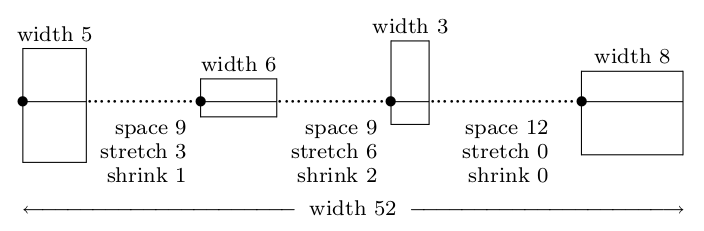
\includegraphics[width=\linewidth ,totalheight=0.95\textheight , keepaspectratio]{glue.png}
\caption{glue说明}
\label{fig:glue说明}
\end{figure}


前面说到盒子的reference point水平排列,然后他们之间还有叫做glue的间距。间距有三个属性:正常间距量(space),拉伸量(stretch),缩减量(shrink)。比如这个图片中第一个glue的正常间距是9个单位,拉伸量为3个单位,缩减量为1个单位。而总的情况是正常间距是5(box1)+9+6+9+3+12\- +8=52个单位。现在假设一行宽58个单位,\TeX 就要调整使得这一行盒子的宽度刚好等于58个单位,于是还需要增加6个单位的宽度,而这6个单位的宽度\footnote{为了简单起见这里不考虑缩减量,具体缩减量如何计算我也不大清楚。}需要从这一行所有glue里的拉伸量中找出来。于是总的拉伸量加法是3+6+0=9。也就是6个单位的宽度要分成9等分再分配给他们,即第一个glue的拉伸量是$3\times\frac { 6 }{ 9 } $。这样第一个间距的总长度就是$9+3\times\frac { 6 }{ 9 } =11$。

经过计算所有的glue间距都确定下来了,那么整个页面布局就确定了。我在这里就戛然而止了,毕竟这里只是对box和glue的基本概念的阐明。


\section{盒子命令介绍}
\href{http://tex.stackexchange.com/questions/83930/what-are-the-different-kinds-of-boxes-in-latex}{参考了这个网站}

\subsection{makebox}
\verb+\makebox[width][allignment]{some text}+\\
还有一个mbox,不过makebox命令更加全面,推荐使用。makebox就是制造一个水平的盒子,注意这个box里面的文本是不能换行的,也就是一行之内的盒子。第一个可选项width指这个盒子的长度,第二个可选项allignment是里面文本的对齐方式,有【l c r s】几个选项,\emph{l}表示左对齐;\emph{c}表示居中;\emph{r}表示right;\emph{s}表示两端对齐。



\subsection{raisebox}
raisebox命令一般的用法就是:\\
\verb+\raisebox{高度}{内容}+\\
表示把某个内容放进一个盒子里然后抬高多少高度,高度值可以是负值则是降低。

\subsection{resizebox}
\href{http://tex.stackexchange.com/questions/13460/scalebox-knowing-how-much-it-scales}{参照了这个网站}

resizebox命令是由graphics宏包提供的,一般都加载了吧。比如tikz绘图的时候如果你只是简单scale那么node内容会出现很大的偏差。这个时候如果你使用scalebox命令则可以将整个图片进行大小变换。

用法如下:\\
\verb+\resizebox{宽度}{高度}{内容} +\\
\verb+\resizebox{\linewidth}{!}{内容}+\\
\verb+\scalebox{2}{测试文字}+

第二个的用法是将这个图片放大到文本宽度,高度填“!”符号的意思是随之而变化。



\subsection{parbox和minipage}
parbox用法:\\
\verb+\parbox[pos][height][contentpos]{width}{text}+

minipage用法:
\begin{Verbatim}
\begin{minipage}[pos][height][contentpos]{width}
text
\end{minipage} 
\end{Verbatim}

他们的参数都类似,具体说明如下:
\begin{description}
\item[pos] \textbf{c}enter,\textbf{t}op和\textbf{b}ottom,说是控制盒子相对周围文本内容的位置。
\item[height] 盒子高度
\item[contentpos] \textbf{c}enter,\textbf{b}ottom,\textbf{t}op,\textbf{s}pread。文本分布,居中,底部,顶部或两端对齐。
\end{description}


\section{带颜色或者线框的盒子}
\subsection{framebox}
framebox和makebox命令类似,除了加上了一个线框。\\
\verb+\setlength{\fboxsep}{10pt}+\\
\verb+\setlength{\fboxrule}{5pt}+\\
如上面描述的这里有两个长度量,fboxsep控制线框和文字之间的距离,fboxrule控制线框的宽度。值得一提的是framebox,fbox 或者fcolorbox命令的线框的这两个参数都是类似上面的代码控制的。


\subsection{colorbox}
colorbox,带颜色的盒子。第一个参数是背景颜色,第二个参数是盒子里面的内容。

\begin{Verbatim}
\colorbox{yellow!50}{this is a test line.}
\end{Verbatim}

\begin{figure}[H]
\centering
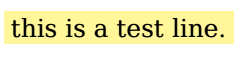
\includegraphics[scale=1 , keepaspectratio]{colorbox.png}
\end{figure}


\subsection{fcolorbox}
fcolorbox和colorbox的区别就是外面加了一个边框,然后第一个参数是边框的颜色,第二个参数是背景颜色,第三个参数是盒子里面的内容。

\begin{Verbatim}
\fcolorbox{red!50}{yellow!30}{this is a test line.}
\end{Verbatim}

\begin{figure}[H]
\centering

\includegraphics[scale=1 , keepaspectratio]{fcolorbox.png}
\end{figure}


\section{保存盒子}
\subsection{savebox}


\chapter{线条}
\verb+\rule[depth]{width}{height}+
这三个选项都要填长度量,第一个长度量是线条竖向偏移量,第二个长度量是线条横向长度,第三个长度量是线条竖向宽度。

\chapter{大文档管理}
之前我也用过include命令来试着将文档分开,但是发现一是减弱了编辑器的各种小插件功能,二是有的时候include命令会出错(一些奇怪的错误,我也不太明白)。然后那个includeonly命令我觉得也挺累赘的,如果你使用input命令,不要引入了前面加个百分号注释掉即可。一个文档就是整体,觉得还是不要分开的好。




\part{xelatex应用篇}
\chapter{tikz制图}
tikz制图我折腾过一段时间,\href{https://github.com/a358003542/tikz_gallery}{这个项目} 读者可以看下。

\chapter{化学相关}
化学相关符号甚至非常复杂的有机分子式的显示问题推荐用\emph{chemfig}宏包解决。


\chapter{exam类}
详细情况请参看本github中文件夹 \verb+exam类+ 。

\chapter{beamer类}
\LaTeX 中幻灯片的处理是用beamer类来写的,老实说我认为\LaTeX 并不适合偏视觉的幻灯片的编写,\LaTeX 更适合内容文字等等较多的时候的情况,那个时候 word都有点力不从心,而tex标记语法风格结合良好的编辑器是很得心应手的。

所以这部分内容我决定略过了,在本github里面有个 \verb+制作幻灯片+ 的文件夹,里面有一点我早期探索的内容,可做读者的参考。




\appendix
\part{附录}


\chapter{windows下作业}
windows安装其实还更简单一些,就是搜索 \emph{texlive} 然后安装之即可。

推荐把texmaker也下载下来安装好,然后其编译命令本文已有所叙述,大体是:
\begin{Verbatim}
xelatex -synctex=1 -interaction=nonstopmode --enable-write18 %.tex
\end{Verbatim}

其中minted宏包需要你安装好python环境,然后用pip安装pygments。然后下面是一些重要的注意事项:

\section{windows下作业请注意}
\begin{itemize}
\item 图片名字,本tex文件名字和重要的文件夹名字都必须使用拼音或英文,不能带中文字符!
\item 其他的都还好吧。
\end{itemize}


\section{windows下安装字体}
双击打开字体文件,右边就有个安装字体按钮。


\chapter{ubuntu下作业}
\section{配置\LaTeX 编写环境}
\label{sec-8}
\begin{enumerate}
\item sudo apt-get install texlive   (下载安装有名的texlive)
\item sudo apt-get install texlive-full   (下载安装texlive的各个包)
\item 在ubuntu软件中心中下载安装texmaker软件。
\item 在texmaker的选项和配置texmaker里面 (现在texmaker已经加入XeLaTeX 编译命令。),设置快速构建,点上用户自定义那一栏,然后输入如下命令:
\end{enumerate}

\begin{Verbatim}
xelatex -interaction=nonstopmode \%.tex|
\end{Verbatim}

这是使用xelatex来对目标tex文件进行编译,而不是传统的latex或者pdflatex方式,之所以这样是因为多方对比之后,觉得其在字体处理方面是未来的趋势。


\section{ubuntu安装字体}
\subsection{找字体文件}
如果你装了windows系统,那么你可以到windows下copy这些字体文件。比如windows常用的宋体,times new roman等,在C盘的windows的fonts文件夹里面。本文用的就是adobe中文系列:adobe 宋体 std, adobe 黑体 std , adobe 楷体 std 。

或者去网络上下载。

\subsection{放置字体文件}

推荐都放在ubuntu的主目录的 \verb+.fonts+ 文件夹里面(这是一个隐藏目录),如果没有请新建一个。这是通常默认用户新加字体放置的目录。

\subsection{安装字体}

运行命令:
\begin{minted}{bash}
fc-cache -f  -v
\end{minted}


字体就安装好了,如果你要看现在你的系统上有那些可用的中文字体,在终端运行命令:
\begin{minted}{bash}
fc-list :lang=zh | sort >ziti.txt
\end{minted}

   
\verb+|+ 表示linux命令中的通道,第一个命令的输出信息流会流向sort命令,排序之后重定向到ziti.txt文件里面。然后终端的数据就保存在这个文件里面了。

打开ziti.txt,里面就是你的可用中文字体的信息,比如:
\begin{Verbatim}
/home/wanze/.fonts/simsun.ttc:  宋体,SimSun:style=Regular
\end{Verbatim}
    
其中第一个是字体文件所在的目录,第二个信息是可以调用的名字,有宋体和SimSun。





\section{新宏包的安装}
\label{sec-9}
安装texlive-full之后,如果还遇到没有的宏包,可以先到CTAN官网上下载到这个宏包之后,然后将这个宏包解压到系统目录: \verb~/usr/share/texmf/tex/latex~ 里面即可。

当然你也可以在另外一个文件夹里面,这里必须是你的主文件夹下,新建一个文件夹texmf,然后里面新建一个tex,然后再新建一个目录latex,然后在这个latex里面放着你下载下来的宏包。具体比如说有一个宏包名字叫做config,那么latex下面就是config文件夹,然后里面就是config.sty文件。你自己写的宏包扔进去一样有效。
唯一要额外做的操作就是在texmf目录之下运行命令:
\begin{minted}{text}
sudo texhash
\end{minted}



让texlive把这个目录也加入搜索范围。


\subsection{阅读宏包代码}
\label{sec-9-1}
你所接触到的latex宏包源码大多在目录:
\begin{Verbatim}
/usr/share/texlive/texmf-dist/tex/latex
\end{Verbatim}


如果有需要的可以阅读这些代码来学习你正在的sty或者cls文件都是怎么编写的。其中base文件夹里面有book,article,report之类文档类型的定义,也许里面有些命令的原始代码是你需要的。

\chapter{利用pandoc输出epub}
\label{ch:pandoc_epub}
一个总的原则就是不要使用太过于花哨的latex特性,请参看本书xelatex基础篇部分,其中讨论的内容基本上latex和epub两边都能兼顾得很好,可能epub那边想要显示的样式会没有,比如你定制了一个自己的罗列环境标签,而在epub那边则总是 \verb+1.+ 之类的,因为epub里面的内容实质上是html,所以这可以通过css来进一步调整,问题不是太大。下面更详细地讨论一些具体的问题。

\begin{itemize}
\item 图片格式不要选pdf和svg了,就用png或者jpeg,然后图片类型后缀名不要省略了。
\item 不要使用 \XeLaTeX 和 \XeTeX ,epub那边不支持
\item 图表环境下label应该跟在caption后面,否则epub那边工作不正常,原因不明。
\item 数学模式基本上都支持,其在epub中大概是这样的形式 \verb+<math ....+,还可以换成mathjax,关于这块pandoc文档的 \verb+Math rendering in html+ 一节有更详细的讨论,不管怎么说,默认的配置一般就够用了。
\item cite命令和参考文献环境thebibliography都工作不太正常。
\item 自定义命令和自定义环境的宏展开pandoc都是支持的,经过测试发现\textbf{可选参数形式不支持}。
\item verbatim和Verbatim环境都是支持的,将转成html那边的pre标签,minted环境的语法高亮也是支持的,同样需要你安装pygments。
\end{itemize}

最终制作epub输出命令简单如下:
\begin{Verbatim}
pandoc -o main.epub main.tex --metadata-file=epub.yaml
\end{Verbatim}



\chapter{方便手机上观看的pdf}


\section{geometry修改}
手机上看旁注,左右上下边距都要缩小,然后paperwidth和paperheight也要相应缩小。本小节 \footnote{主要参考了\href{http://tex.stackexchange.com/questions/78920/generating-smartphone-readable-pdf}{这个网站}。}

\begin{Verbatim}
\ifphone
%for phone
\RequirePackage[
  paperwidth=105mm, %除去旁註其他沒變,115,再稍微小點
  paperheight=190mm,%太長了縮短點,
  bindingoffset=0mm,%裝訂線
  top=15mm,  %上邊距 包括頁眉
  bottom=15mm,%下邊距 包括頁腳
  left=5mm,  %左邊距or inner
  right=5mm,  %右邊距or  outer
  headheight=10mm,%頁眉
  footskip=10mm,%頁腳
  includemp=true,% 旁註寬度計入width
  marginparsep=0mm, %沒有旁註
  marginparwidth=0mm,  %沒有旁註
  ]{geometry}
\else

\RequirePackage[a4paper, %a4paper size 297:210 mm
  bindingoffset=0mm,%裝訂線
  top=45mm,  %上邊距 包括頁眉
  bottom=40mm,%下邊距 包括頁腳
  left=35mm,  %左邊距or inner
  right=40mm,  %右邊距or  outer
  headheight=25mm,%頁眉
  footskip=25mm,%頁腳
 includemp=true,% 旁註寬度計入width
 marginparsep=0mm, %旁註與正文間距
marginparwidth=0mm,  %旁註寬度
  ]{geometry}
\fi
\end{Verbatim}
这里使用了一个条件命令。在加载myconfig.sty宏包的时候已经新建了一个条件变量:\\
\verb+\newif\ifphone+\\
\verb+\phonefalse+
ifphone就是一个条件判断命令,这里涉及到的命令我也不大懂,总之,如果我改成:\\
\verb+\phonetrue+\\
就会自动生成适合在手机上观看的pdf。



\section{章节上下距离修改}
使用 \verb+titlespacing*+ 来修改章节的上下距离,经观察主要是chapter和secion上下间距较大。 \verb+titlespacing*+ 命令第一个参数是指定作用对象,第二个指定左边距离,第三个是指定上间距,第四个是指定下间距。 参考了 \href{https://tex.stackexchange.com/questions/63390/how-to-decrease-spacing-before-chapter-title}{这个网页}。

\begin{Verbatim}
\titlespacing*{\chapter}{0pt}{-45pt}{10pt}

\titlespacing*{\section}{0pt}{-5pt}{8pt}
\end{Verbatim}



\section{管理策略}
手机版和电脑版sty文件分开编写和引入是个不错的主意,至于具体生成的pdf文件名字后面再重命名就是了。



\chapter{其他问题的讨论}

\section{TeX一些常用命令简介}
如果读者真的要学习TeX原生命令,推荐查阅\href{http://www.tug.org/utilities/plain/cseq.html}{这个网站} 和阅读高德纳写的 The TexBook。

\subsection{relax命令}
类似python的pass命令,什么也不做的意思。

\section{TeX中执行系统的命令}
\href{http://tex.stackexchange.com/questions/20444/what-are-immediate-write18-and-how-does-one-use-them}{参考了这个网站}

\TeX 的write18命令将一连串文本命令送入shell中执行,一般语句的格式如下(immediate命令是立即执行的意思。这里表示将命令立即送入shell现在就执行。):\\
\verb+\immediate\write18{your command put it here}+

要成功运行这个命令记得你的编译选项上还需要加上:\\
\verb+--enable-write18+

比如目前我的texmaker的编译命令如下:
\begin{Verbatim}
xelatex -synctex=1 -interaction=nonstopmode 
    --enable-write18  %.tex
\end{Verbatim}


\section{TeX中写文件和读文件}
\href{http://stackoverflow.com/questions/2115379/write-and-read-from-a-latex-temporary-file}{参考了这个网站}

TeX中写文件的流程如下: 
\begin{enumerate}
\item 首先新建一个待写的文件:\\
\verb+\newwrite\tempfile+
\item 然后打开这个文件并给这个文件一个实际的文件名(支持带文件夹的相对路径名前缀):\\
\verb+\immediate\openout\tempfile=test.txt+
\item 然后用write命令给这个文件写入信息,只要文件没有关闭,可以一直附加的写:\\
\verb+\immediate\write\tempfile{this is interesting}+
\item 写完之后记得关闭文件,这样写入的内容才实际从缓存区进入真实的文件区:\\
\verb+\immediate\closeout\tempfile+
\end{enumerate}

TeX中读入文件一般用input命令即可,此外verbatim宏包还提供了原文照列的verbatiminput命令,还有fancyvrb宏包有Verbatiminput命令。

\section{TeX中的程序结构}
\subsection{条件控制语句}
\label{sec:条件控制语句}
\href{http://handyfloss.wordpress.com/2007/08/29/latex-programming-how-to-implement-conditionals/}{参考了这个网站}

条件控制语句的首先要新建一个条件控制变量:\\
\verb+\newif\iflogvar+
默认这个变量是设置为假,然后通过以下模式来建立条件语句:
\begin{Verbatim}
\iflogvar
  aaaa
\else
  bbbb
\fi
\end{Verbatim}
条件语句可以嵌套,然后你可以通过这样的命令来调整条件控制变量的真假:\\
\verb+\logvartrue+\\
\verb+\logvarfalse+

\subsubsection{ifnum命令}
ifnum命令用于判断数字。\\
\verb+\ifnum number = 0+\\
ifnum控制结构和if命令类似,这里数字判断还可以是大于>或者小于<。

\section{TeX生成前面有零的数字序列}
\href{http://tex.stackexchange.com/questions/30930/how-to-output-a-counter-with-leading-zeros}{参考了这个网站}

TeX中的计数器用arabic命令之后是1 2 3...这样的形式,如何产生001 002... 010 011 ... 100 ...这样的形式呢?之所以有这样的需求是我在试着编写endnotes宏包的时候用了一种错误的思路,然后希望使用linux系统的cat命令来讲一条条的尾注汇总,cat命令对于计数器产生的文件名,如果按照原来1 2 3...这样的形式顺序是错误的,为了纠正就需要变成001  002 ...这样的一致规则形式。

\begin{Verbatim}
\def\@entname{\jobname
\ifnum\value{@ShowEndnoteCounter}<10 0\fi
\ifnum\value{@ShowEndnoteCounter}<100 0\fi
\arabic{@ShowEndnoteCounter}}%
\end{Verbatim}

比如上面这个命令,就是我目前使用的endnotes宏包产生的临时ent文件,文件名如下:xelatex指南001.ent xelatex指南002.ent等等。

这里的逻辑如下,首先假定这个计数器从0开始吧,小于0的情况不予考虑,不要视图做出什么情况都考虑到的完美程序,那只是浪费脑力罢了。如果计数器范围在0到9,那么经过第二行将会生成一个0,经过第三行将会生成另外一个0,然后后面生成个位数的计数器1之类的。如果计数器范围10到99,那么经过第二行不会生成0什么也没有,如是格式就有了010 011之类的。这种构造考虑程序自上而下的顺序,很是简单,比如你如果觉得一千之类的范围太小,那就再加上类似的一行。



\section{文本中的上标还有下标}
上标使用命令textsuperscript命令,下标感觉自己缩小点就差不多了吧。示例如下:\\
上标\textsuperscript{上标}下标{\scriptsize 下标}

更常见的是化学分子式里面的上标和下标,推荐使用mhchem宏包,至于数学模式里的上标和下标自不必说了。


\section{定制quote和quoation环境}
以下讨论参考了\href{http://tex.stackexchange.com/questions/33219/whats-the-difference-between-the-environments-quote-and-quotation}{这个网站} 。

quote和quotation在article.cls中的原初定义是这样的:
\begin{Verbatim}
\newenvironment{quote}
               {\list{}{\rightmargin\leftmargin}%
                \item\relax}
               {\endlist}
\newenvironment{quotation}
               {\list{}{\listparindent 1.5em%
                        \itemindent    \listparindent
                        \rightmargin   \leftmargin
                        \parsep        \z@ \@plus\p@}%
                \item\relax}
               {\endlist}
\end{Verbatim}

我改成了如下:
\begin{Verbatim}
%=========重新定义 quote=====%
\renewenvironment{quote}[1][anonymous]{
\newcommand{\quoteauthor}[1][anonymous]{#1}
\list{}{\rightmargin\leftmargin %右间距等于左间距
\itemindent   2em
}\item\relax
\ttfamily}
{\\
\makebox[\linewidth][r]{\sffamily —\quoteauthor}
\endlist}

%重新定义quotation
\renewenvironment{quotation}
{\list{}{\rightmargin\leftmargin %右间距等于左间距
\itemindent 2em%item的缩进也就是第一段的缩进
\listparindent \itemindent %第二段的缩进
}%
\item\relax
\ttfamily}
{\endlist}
\end{Verbatim}
quote和quotation都是通过list环境来实现的,具体不太清楚。这里就我做的修改说明如下:
\begin{itemize}
\item \verb+\rightmargin\leftmargin+这是让右边空白距离等于左边空白距离,左边空白距离默认等于\verb+\parindent+,这个有用我保留了。
\item \verb+\itemindent   2em+,这个itemindent控制的是第一段的段首缩进量,这里设置为2em即两个字符的意思。
\item 代码第七行是设置quote环境下字体为ttfamily。
\item quote环境后面的代码,在结束环境之前,先换行,然后输出了一个盒子,右对齐,ssfamily,写着这个格言的作者,因为格言一般都要写上作者,如果不知道那么也写上anonymous,无名氏。这个作者的名字是quote环境接受一个可选项而来的额。
\item \verb+\listparindent \itemindent+,quotation多了一个这个设置,其中listparindent是控制quotation里面除了第一段之外其他段落的缩进,这里就简单设置为跟第一段一样。
\item quotation环境的其他修改,parsep是控制段与段之间距离的,这里取消了,因为默认的就很好了。
\end{itemize}


\section{多张图片并列显示}
\label{sec:多张图片并列显示}

\begin{Verbatim}
\begin{figure}[h]

\label{fig:四栏图片}
\begin{multicols}{4}

\includegraphics[width=\linewidth ,totalheight=\textheight , 
        keepaspectratio]{temp.jpg}
i want  some test to show there is a text and not to column break.\\
\centerline{test}
\columnbreak

\includegraphics[width=\linewidth ,totalheight=\textheight , 
         keepaspectratio]{temp.jpg}
\centerline{test}
\columnbreak

\includegraphics[width=\linewidth ,totalheight=\textheight ,
         keepaspectratio]{temp.jpg}
\centerline{test}
\columnbreak

\includegraphics[width=\linewidth ,totalheight=\textheight ,
         keepaspectratio]{temp.jpg}
\centerline{test}
\end{multicols}
\caption{denosie fig}

\end{figure}
\end{Verbatim}
这段代码的分栏还有插入图片知识都已经介绍了,值得一提的就是widetext环境,也就是有changepage宏包而来的临时改变页面布局环境和浮动体环境figure以及table不兼容。比如放入浮动体环境内才能起作用。然后caption命令似乎只是默认的linewidth居中。所以如果想要图片和表格在扩大的文本布局中居中对齐,那么需要在浮动体环境内部使用改变页面布局命令,然后使用居中命令。

\section[生成字体所有已有的字形]{生成字体所有已有的字形\footnote{主要参照了\href{http://tex.stackexchange.com/questions/23863/generating-a-table-of-glyphs-with-xetex}{这个网站}}}
\label{sec:字体已有字形}
\begin{Verbatim}
\documentclass[landscape]{article}
\usepackage{geometry}
\usepackage{fontspec}
\setmainfont{DejaVu Sans}
\usepackage{multicol}
\setlength{\columnseprule}{0.4pt}
\usepackage{multido}
\setlength{\parindent}{0pt}
\begin{document}
\begin{LARGE}
\begin{multicols}{5}
\multido{\i=0+1}{"10000"}{
  \iffontchar\font\i
    \makebox[4em][l]{\i}%
    \symbol{\i}\endgraf
  \fi
}
\end{multicols}
\end{LARGE}
\end{document}
\end{Verbatim}


\section{临时改变页面布局}
临时改变页面布局前面讲的geometry宏包也有一种实现机制,但是不太好用而且会把后面的段落格式打乱。这里推荐使用changepage宏包。

进入adjustwidth环境就可以调整旁注宽度了。比如这里我新建一个widetext环境代码如下:

\begin{Verbatim}
\newenvironment{widetext}  
	{\begin{adjustwidth}{}{-70mm}}%marginparwidth+marginparsep
	{\end{adjustwidth}}
\end{Verbatim}  

新建环境请看\ref{sec:新的环境}。我们在这里建立了一个widetext环境,主要是adjustwidth环境操作,我们看到后面有两个花括号,第一个指左margin,第二个指右margin。注意这里不要和前面geometry宏包里面设置的includemp弄混了。\footnote{geometry宏包里面设置includemp=true让marginpar部分进入width,也就是right margin并不包含旁注部分了,但是只适用于geometry宏包。}这里左margin就是前面设置的left,右margin是前面设置的:\\right+marginparwidth+marginparsep。所以可以考虑geometry宏包不要设置includemp,我前面只是为了理解简单才如此设置的,当然这里理解这个概念了就没有什么问题了。

然后正数表示margin宽度增大,负数表示margin部分宽度减小。这里设置-70mm即右边marginparwidth+marginparsep的宽度。然后自己注意进入这个环境了就不要使用marginpar或者其他旁注的命令了,这是显而易见的。不设置数值即表示不改变,出了adjustwidth环境,一切复原。

还有一个adjustwidth*环境,意思表示margin改变随着页面奇偶数变化而定,这个宏包的页面奇偶数设定及相关讨论后面都略过了,因为本文只关注于oneside模式,毕竟电子书籍设置成为oneside更好一些。

changepage宏包还有changetext和changepage命令,有兴趣的可以看下,感觉并不太好用。




\backmatter
\chapter*{参考文献}
\addchtoc{参考文献}
\begin{thebibliography}{9}
\bibitem[lshort]{lshort} 有名的《一份不太简短的\LaTeX2e 介绍》,原版作者:Tobias Oetik\- er,Hubert Partl,Irene Hyna等,版本:2001-08-09,中文翻译:CTeX用户小组,版本:2002-05,pdf下载链接:\\ \href{http://www.ctan.org/tex-archive/info/lshort/chinese}{http://www.ctan.org/tex-archive/info/lshort/chinese}。

\bibitem[latex123]{latex123}  《大家来学\LaTeX 》,原版作者:李果正,版本:2004-03-08,网站链接:\href{http://edt1023.sayya.org/tex/latex123/}{http://edt1023.sayya.org/tex/latex123/}。

\bibitem[wikibook-latex]{wikibook-latex} 维基图书latex篇英文版,版本:2013-08,网站链接\\:\href{http://en.wikibooks.org/wiki/LaTeX}{http://en.wikibooks.org/wiki/LaTeX}。\emph{这本书甚至都没有cite它一下,因为不知道插在哪里,几乎到处都有对它的引用,谢谢所有wikibook的编写者。}

\bibitem[boxes]{boxes} using boxes and glue in \TeX{} and \LaTeX ,原版作者:Nelson H. F. Beebe,版本:2009-03-28,pdf下载链接:链接地址不好复制,请google搜索书名之。

\bibitem[latex-companion]{latex-companion}  The Latex Companion 




\end{thebibliography}


\end{document}



